%\setlength{\parindent}{0pt}
\documentclass{article}
\usepackage{amsmath}
\usepackage{amssymb}
\usepackage{amsthm}
\usepackage{latexsym}

\usepackage{amsopn}
\DeclareMathOperator{\stab}{Stab}
\DeclareMathOperator{\perm}{Perm}
\DeclareMathOperator{\im}{im}
\DeclareMathOperator{\Aut}{Aut}
\DeclareMathOperator{\Hom}{Hom}
\DeclareMathOperator{\Perm}{Perm}
\DeclareMathOperator{\Frac}{Frac}
\DeclareMathOperator{\Pic}{Pic}
\DeclareMathOperator{\id}{id}
\DeclareMathOperator{\Tr}{Tr}
\DeclareMathOperator{\Spec}{Spec}
\DeclareMathOperator{\Proj}{Proj}
\DeclareMathOperator{\codim}{codim}


\usepackage[dvipsnames]{xcolor}
 
\definecolor{mypink1}{rgb}{0.858, 0.188, 0.478}


\usepackage{listings}
%\def\lstlanguagefiles{lstlean.tex} 
%\lstset{language=lean}

\usepackage[utf8]{inputenc}
\usepackage{listings}
%\usepackage{xcolor}

\definecolor{codegreen}{rgb}{0,0.6,0}
\definecolor{codegray}{rgb}{0.5,0.5,0.5}
\definecolor{codepurple}{rgb}{0.58,0,0.82}
\definecolor{backcolour}{rgb}{0.95,0.95,0.92}

\lstdefinestyle{pystyle}{
    backgroundcolor=\color{backcolour},   
    commentstyle=\color{codegreen},
    keywordstyle=\color{magenta},
    numberstyle=\tiny\color{codegray},
    stringstyle=\color{codepurple},
    basicstyle=\ttfamily\footnotesize,
    breakatwhitespace=false,         
    breaklines=true,                 
    captionpos=b,                    
    keepspaces=true,                 
    numbers=left,                    
    numbersep=5pt,                  
    showspaces=false,                
    showstringspaces=false,
    showtabs=false,                  
    tabsize=2
}

\usepackage{enumitem}
\usepackage{tikz-cd}

\usepackage{tikz,tkz-euclide}
\usetikzlibrary{arrows,calc,intersections}
%\usetkzobj{all}

\usepackage{enumitem}
\usepackage[margin=2.2cm]{geometry}

\newcommand{\ideal}{\ensuremath{\triangleleft}}
\newcommand{\ol}{\ensuremath{\overline}}
\newcommand{\p}{\ensuremath{\mathfrak{p}}}
\newcommand{\m}{\ensuremath{\mathfrak{m}}}
\newcommand{\A}{\ensuremath{\mathbb{A}}}
\newcommand{\Z}{\ensuremath{\mathbb{Z}}}
\newcommand{\C}{\ensuremath{\mathbb{C}}}
\newcommand{\R}{\ensuremath{\mathbb{R}}}
\newcommand{\Q}{\ensuremath{\mathbb{Q}}}
\newcommand{\N}{\ensuremath{\mathbb{N}}}
\newcommand{\F}{\ensuremath{\mathbb{F}}}
\renewcommand{\P}{\ensuremath{\mathbb{P}}}
\newcommand{\Ox}{\mathscr{O}}

\newcommand{\q}{\ensuremath{\mathfrak{q}}}
%\newcommand{\N}{\ensuremath{\mathbb{N}}}

\usepackage{mathrsfs}
%\usepackage{fontspec}
%\usepackage{mathtools}
%\usepackage{unicode-math}

\usepackage{natbib}
\bibliographystyle{humannat}
%\bibliographystyle{unsrtnat}
%\bibliographystyle{abbrvnat}

\numberwithin{figure}{section}

\theoremstyle{definition}
\newcounter{dummy} \numberwithin{dummy}{section}
\newtheorem{lemma}[dummy]{Lemma}
%\newtheorem*{lemma*}[dummy]{Lemma}
\newtheorem{prop}[dummy]{Proposition}
\newtheorem{defi}[dummy]{Definition}
\newtheorem{cor}[dummy]{Corollary}
\newtheorem{example}[dummy]{Example}
\newtheorem{thm}[dummy]{Theorem}



\newcommand*{\DashedArrow}[1][]{\mathbin{\tikz [baseline=-0.25ex,-latex, dashed,#1] \draw [#1] (0pt,0.5ex) -- (1.3em,0.5ex);}}%
\newcommand{\dto}{\DashedArrow[->,densely dashed]}
%\newcommand{\da}{\DashedArrow}

%\usepackage{microtype}
\usepackage[activate={true,nocompatibility},final,tracking=true,kerning=true,spacing=true,factor=1100,stretch=10,shrink=10]{microtype}
\author{Louis Carlin -- u6384109}
\title{World Models with MDRNNs}
\usepackage[pdftex]{hyperref}
\hypersetup{
  colorlinks=true
}
\begin{document}
\maketitle
\begin{abstract}
The paper World Models \citep{ha2018world} describes an architecture allowing a computer agent to learn an internal model of its own environment.
This model was powerful enough that agents could be trained in its dreamed simulation to achieve good performance in the original environment.
In this project I set out to create my own implementation of the World Models architecture.

\end{abstract}

\section{Introduction}
%background stuff of other world models
When humans make decisions we often use an internal model of the problem at hand to inform our decision, allowing us to predict or calculate how the world might unfold based on our actions.
This model based approach may be something we are conscious of, as in the case of a chess player who uses their knowledge to look ahead and evaluate potential moves.
It also happens unconsciously, for example with batters in baseball who use an internal model to infer the position of the ball based on the the way the pitcher throws it, rather than reacting to the position of the ball milliseconds before it hits their bat.
In either case this internal model greatly improves our performance at these tasks.

% \begin{figure}[h]
%   \centering
%   \includegraphics[scale=0.2]{pitch.jpeg}

% \end{figure}

In reinforcement learning we seek to develop computer agents which are capable of \textit{learning} to complete tasks.
Inspired by the success of own model-based thought process we naturally seek to equip these agents with models of their environment.
There are several different ways this has been done.
Most traditionally an agent may be supplied with a model which has been handcrafted by a human. %TODO example
Unfortunately models made in this way are usually domain specific and thus the approach requires significant human involvement any time we try adapt an agent to learn in a new environment.
In a complex or partially unobservable environment it may even be infeasible for a human to equip an agent with a model adequately describing its world. %example?
More recently, deep reinforcement learning has circumvented this problem by increasing the complexity of the learned agent.
Agents constructed using architectures such as recurrent neural networks (RNNs) learn to perform complex computations.
In many cases they are able to harness this power to essentially learn their own model of the environment, allowing them to succeed at complex tasks without human intervention.
Deep reinforcement learning is not a complete solution however: training of complex agents is notoriously difficult, with what is known as the \textit{Credit Assignment Problem} \citep{minsky1961steps} making it difficult to determine which particular actions may have led to a reward.
A third approach, championed by Schmidhuber (\citeyear{schmidhuber1990making}, \citeyear{schmidhuber1990line} \citeyear{schmidhuber1991possibility}, \citeyear{schmidhuber1991reinforcement}, \citeyear{schmidhuber2015learning}) is to decouple the learning process, first learning a model $M$ and then using this model to train a controller $C$.
The advantage of this approach is that complex models can be learned without worrying about credit assignment, allowing us to more easily train a comparatively simple controller.

World Models \citep{ha2018world} is a particularly simple implementation of Schmidhuber's model-controller idea which has been shown to be remarkable effective at learning in simple image-based environments.
The most striking feature of World Models is the power of its learned internal model, which is able to simulate an interactive \textit{dream} of the original environment.
Alongside the original paper David Ha et al. released a \href{https://worldmodels.github.io/}{browser-based version} of these dreams which is definitely worth trying if you haven't seen it already.
In addition to being visually impressive the dreams are stable and accurate enough that agents could be trained entirely enside their own dreams to perform well in the original environment.
In part due to the sheer beauty of the dreams this report focuses more on the internal model than the end-to-end trained agent, however it should be noted that the end-to-end agent is also significant and that the World Models agent was able to achieve record performance in one of the environments it was tested in.

%While the end-to-end World Models agent was able to achieve state of the art performance 

% It breaks an agent into three components, the first two are Vision $V$ and Memory $M$, and together these allow an agent to interpret and model its world.
% The Controller $C$ is then trained using both features of the environment and some of the internal knowledge of $M$.
% Significantly, the internal model comprised of $V$ and $M$ is powerful enough to recreate a simulated version of the original environment, known as a \textit{dream}.
% These dreams were close enough to the original environment that agents could be trained entirely inside a dream to perform well in the original environment.
% In this project I primarily set out to investigate this part of World Models, which consists of the $V$ and $M$ components.

My project was to reimpliment the World Models architecture and to explore its use in different environments.
The original intention was to experiment to see if the internal model could learn to simulate dynamics of more complex environments, but this got somewhat cut short due to time constraints.
The structure of this report is as follows.
We begin with a brief overview of the World Models' architecture which serves as the primary motivation throughout this report.
In the subsequent three sections we discuss some of the theory behind each of the three components of World Models.
Finally, in the last section I discuss my own implementation and results.

\section{The World Models' Architecture}
%\subsection{Problem Description}
World Models uses a fairly standard description of the reinforcement learning problem.
Environments are broken down into discrete time steps.
At a timestep $t$ an agent receives a partial observation of the environment $o_t$ and are reward $r_t$.
The agent must then choose an action $a_t$ from a set of possible actions.
In an \textit{episodic} task where there are only ever finitely many time steps the agent's task is to pick $a_t$ such that the sum of future rewards is maximised.
In a \textit{continuing} task where the environment is ongoing an agent instead picks $a_t$ to maximise a weighted sum of future rewards where more distant rewards are weighted with decreasing values to ensure the sum converges.

Although Schmidhuber's concept of a separate internal model and controller apply more generally, the World Models architecture is adapted to image based problems where the observation $o_t$ is a two dimensional image.
Environments such as these are navigated with ease by humans playing videogames, yet still remain a challenge in reinforcement learning.
Ha and Schmidhuber tested their model in two different environments.
The first one was \texttt{CarRacing-v0} \citep{carRacing} where an agent must learn to drive a car based on a top-down image of the racing track.
Here the agent is rewarded more the more tiles they visit, which incentivises speedier and more accurate driving.
The second environment was \texttt{VizDoom: Take Cover} \citep{kempka2016vizdoom} where an agent learns to dodge fireballs thrown at it by demons in the 3D environment of the videogame Doom.
In this environment observations are first person images from the perspective of the agent and rewards are simply given to the agent based on survival time.
%TODO picture of both environments

\begin{figure}[h]
  \centering
  \begin{minipage}{0.45\textwidth}
      \centering
      \includegraphics[width=0.9\textwidth]{CarRacing-v0.jpeg} % first figure itself
      \caption{An observation from the \texttt{CarRacing-v0} environment}
  \end{minipage}\hfill
  \begin{minipage}{0.45\textwidth}
      \centering
      \includegraphics[width=0.9\textwidth]{VizDoom.jpeg} % second figure itself
      \caption{An observation from the \texttt{VizDoom: Take Cover} environment}
  \end{minipage}
\end{figure}

%overview of model V-M-C
The World Models' architecture is split into three components: \textit{Vision (V), Memory (M)}, and \textit{Controller (C)}.
These models are trained in order as each one depends on the learned knowledge of the previous components.
The Vision component %is comprised of an variational autoencoder.
takes in an image observation $o_t$ and gives a much smaller vector $z_t$, known as the \textit{latent state}, which we can think of as a compressed version of $o_t$.
The idea behind this compression is that it will be easier to learn an internal model of the dynamics of this smaller latent state than to try predict the evolution of the observation images. 
The Memory component forms the bulk of agent's internal model.
Given the current latent state $z_t$, an action $a_t$, and its own memory output $h_{t}$ from the previous state, $M$ is trained to predict the distribution of what the next latent state $z_{t+1}$ will be given that action.
That is, $M$ learns the distribution $p(z_{t+1} | z_t, a_t, h_t)$, which we think of as the rules of how the environment evolves.
Finally, the Controller is trained to choose the optimal action $a_t$ based on both the current latent state $z_t$ given to it by $V$ and the internal state $h_{t-1}$ from $M$. 

\begin{figure}[h]
  \centering


\tikzset{every picture/.style={line width=0.75pt}} %set default line width to 0.75pt        

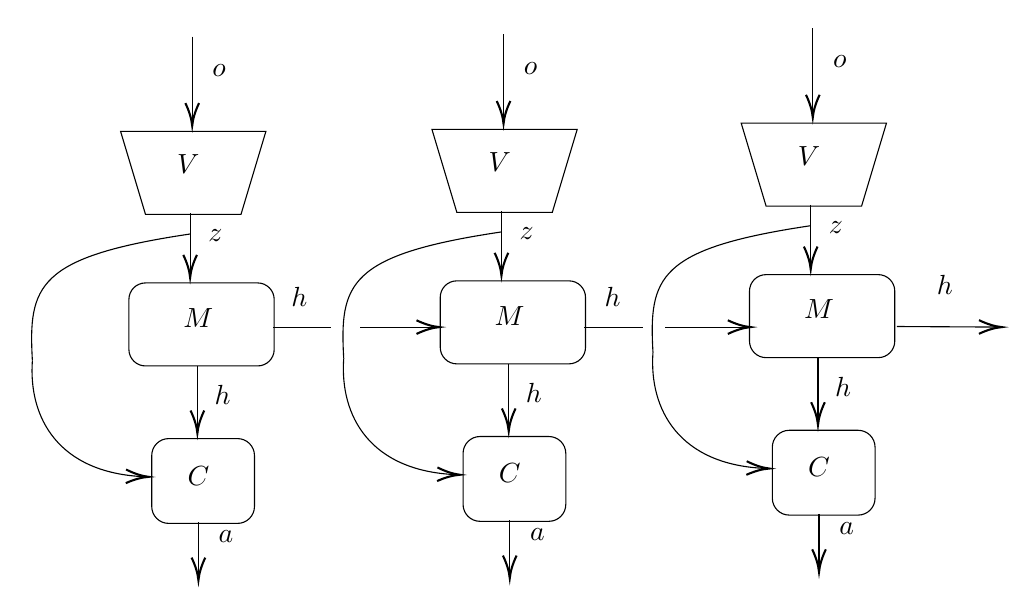
\begin{tikzpicture}[x=0.75pt,y=0.75pt,yscale=-1,xscale=1]
%uncomment if require: \path (0,300); %set diagram left start at 0, and has height of 300

%Shape: Trapezoid [id:dp8835259262509831] 
\draw   (214,73) -- (202,113) -- (156,113) -- (144,73) -- cycle ;
%Rounded Rect [id:dp0285219553359235] 
\draw   (148,154) .. controls (148,149.58) and (151.58,146) .. (156,146) -- (210,146) .. controls (214.42,146) and (218,149.58) .. (218,154) -- (218,178) .. controls (218,182.42) and (214.42,186) .. (210,186) -- (156,186) .. controls (151.58,186) and (148,182.42) .. (148,178) -- cycle ;
%Rounded Rect [id:dp3457403063059383] 
\draw   (159,229.17) .. controls (159,224.66) and (162.66,221) .. (167.17,221) -- (200.33,221) .. controls (204.84,221) and (208.5,224.66) .. (208.5,229.17) -- (208.5,253.69) .. controls (208.5,258.2) and (204.84,261.86) .. (200.33,261.86) -- (167.17,261.86) .. controls (162.66,261.86) and (159,258.2) .. (159,253.69) -- cycle ;
%Straight Lines [id:da5830231307220126] 
\draw    (181,186) -- (181,216.43) ;
\draw [shift={(181,218.43)}, rotate = 270] [color={rgb, 255:red, 0; green, 0; blue, 0 }  ][line width=0.75]    (10.93,-3.29) .. controls (6.95,-1.4) and (3.31,-0.3) .. (0,0) .. controls (3.31,0.3) and (6.95,1.4) .. (10.93,3.29)   ;
%Straight Lines [id:da21875827228445366] 
\draw    (177.5,112.43) -- (177.5,141.43) ;
\draw [shift={(177.5,143.43)}, rotate = 270] [color={rgb, 255:red, 0; green, 0; blue, 0 }  ][line width=0.75]    (10.93,-3.29) .. controls (6.95,-1.4) and (3.31,-0.3) .. (0,0) .. controls (3.31,0.3) and (6.95,1.4) .. (10.93,3.29)   ;
%Curve Lines [id:da18494477060365933] 
\draw    (177.5,122.43) .. controls (103.5,133.43) and (99.5,147.43) .. (101.5,183.43) ;
%Curve Lines [id:da3167428765764193] 
\draw    (101.5,183.43) .. controls (99.53,211.01) and (114.05,237.62) .. (155.58,239.37) ;
\draw [shift={(157.5,239.43)}, rotate = 181.33] [color={rgb, 255:red, 0; green, 0; blue, 0 }  ][line width=0.75]    (10.93,-3.29) .. controls (6.95,-1.4) and (3.31,-0.3) .. (0,0) .. controls (3.31,0.3) and (6.95,1.4) .. (10.93,3.29)   ;
%Straight Lines [id:da13659803234644108] 
\draw    (178.5,27.29) -- (178.5,68.29) ;
\draw [shift={(178.5,70.29)}, rotate = 270] [color={rgb, 255:red, 0; green, 0; blue, 0 }  ][line width=0.75]    (10.93,-3.29) .. controls (6.95,-1.4) and (3.31,-0.3) .. (0,0) .. controls (3.31,0.3) and (6.95,1.4) .. (10.93,3.29)   ;
%Straight Lines [id:da7386372433419905] 
\draw    (181.5,261.29) -- (181.5,287.29) ;
\draw [shift={(181.5,289.29)}, rotate = 270] [color={rgb, 255:red, 0; green, 0; blue, 0 }  ][line width=0.75]    (10.93,-3.29) .. controls (6.95,-1.4) and (3.31,-0.3) .. (0,0) .. controls (3.31,0.3) and (6.95,1.4) .. (10.93,3.29)   ;
%Shape: Trapezoid [id:dp1462361877942473] 
\draw   (364,72) -- (352,112) -- (306,112) -- (294,72) -- cycle ;
%Rounded Rect [id:dp18606077574272506] 
\draw   (298,153) .. controls (298,148.58) and (301.58,145) .. (306,145) -- (360,145) .. controls (364.42,145) and (368,148.58) .. (368,153) -- (368,177) .. controls (368,181.42) and (364.42,185) .. (360,185) -- (306,185) .. controls (301.58,185) and (298,181.42) .. (298,177) -- cycle ;
%Rounded Rect [id:dp4652776111951933] 
\draw   (309,228.17) .. controls (309,223.66) and (312.66,220) .. (317.17,220) -- (350.33,220) .. controls (354.84,220) and (358.5,223.66) .. (358.5,228.17) -- (358.5,252.69) .. controls (358.5,257.2) and (354.84,260.86) .. (350.33,260.86) -- (317.17,260.86) .. controls (312.66,260.86) and (309,257.2) .. (309,252.69) -- cycle ;
%Straight Lines [id:da9151430963452045] 
\draw    (331,185) -- (331,215.43) ;
\draw [shift={(331,217.43)}, rotate = 270] [color={rgb, 255:red, 0; green, 0; blue, 0 }  ][line width=0.75]    (10.93,-3.29) .. controls (6.95,-1.4) and (3.31,-0.3) .. (0,0) .. controls (3.31,0.3) and (6.95,1.4) .. (10.93,3.29)   ;
%Straight Lines [id:da07699090937850928] 
\draw    (327.5,111.43) -- (327.5,140.43) ;
\draw [shift={(327.5,142.43)}, rotate = 270] [color={rgb, 255:red, 0; green, 0; blue, 0 }  ][line width=0.75]    (10.93,-3.29) .. controls (6.95,-1.4) and (3.31,-0.3) .. (0,0) .. controls (3.31,0.3) and (6.95,1.4) .. (10.93,3.29)   ;
%Curve Lines [id:da8115724577514165] 
\draw    (327.5,121.43) .. controls (253.5,132.43) and (249.5,146.43) .. (251.5,182.43) ;
%Curve Lines [id:da6705210586592285] 
\draw    (251.5,182.43) .. controls (249.53,210.01) and (264.05,236.62) .. (305.58,238.37) ;
\draw [shift={(307.5,238.43)}, rotate = 181.33] [color={rgb, 255:red, 0; green, 0; blue, 0 }  ][line width=0.75]    (10.93,-3.29) .. controls (6.95,-1.4) and (3.31,-0.3) .. (0,0) .. controls (3.31,0.3) and (6.95,1.4) .. (10.93,3.29)   ;
%Straight Lines [id:da2713335277085913] 
\draw    (328.5,26.29) -- (328.5,67.29) ;
\draw [shift={(328.5,69.29)}, rotate = 270] [color={rgb, 255:red, 0; green, 0; blue, 0 }  ][line width=0.75]    (10.93,-3.29) .. controls (6.95,-1.4) and (3.31,-0.3) .. (0,0) .. controls (3.31,0.3) and (6.95,1.4) .. (10.93,3.29)   ;
%Straight Lines [id:da018255342957326226] 
\draw    (331.5,260.29) -- (331.5,286.29) ;
\draw [shift={(331.5,288.29)}, rotate = 270] [color={rgb, 255:red, 0; green, 0; blue, 0 }  ][line width=0.75]    (10.93,-3.29) .. controls (6.95,-1.4) and (3.31,-0.3) .. (0,0) .. controls (3.31,0.3) and (6.95,1.4) .. (10.93,3.29)   ;
%Shape: Trapezoid [id:dp2430591295177642] 
\draw   (513,69) -- (501,109) -- (455,109) -- (443,69) -- cycle ;
%Rounded Rect [id:dp39814637506948647] 
\draw   (447,150) .. controls (447,145.58) and (450.58,142) .. (455,142) -- (509,142) .. controls (513.42,142) and (517,145.58) .. (517,150) -- (517,174) .. controls (517,178.42) and (513.42,182) .. (509,182) -- (455,182) .. controls (450.58,182) and (447,178.42) .. (447,174) -- cycle ;
%Rounded Rect [id:dp21706991468861547] 
\draw   (458,225.17) .. controls (458,220.66) and (461.66,217) .. (466.17,217) -- (499.33,217) .. controls (503.84,217) and (507.5,220.66) .. (507.5,225.17) -- (507.5,249.69) .. controls (507.5,254.2) and (503.84,257.86) .. (499.33,257.86) -- (466.17,257.86) .. controls (461.66,257.86) and (458,254.2) .. (458,249.69) -- cycle ;
%Straight Lines [id:da2885218987388809] 
\draw    (480,182) -- (480,212.43) ;
\draw [shift={(480,214.43)}, rotate = 270] [color={rgb, 255:red, 0; green, 0; blue, 0 }  ][line width=0.75]    (10.93,-3.29) .. controls (6.95,-1.4) and (3.31,-0.3) .. (0,0) .. controls (3.31,0.3) and (6.95,1.4) .. (10.93,3.29)   ;
%Straight Lines [id:da415487537189946] 
\draw    (476.5,108.43) -- (476.5,137.43) ;
\draw [shift={(476.5,139.43)}, rotate = 270] [color={rgb, 255:red, 0; green, 0; blue, 0 }  ][line width=0.75]    (10.93,-3.29) .. controls (6.95,-1.4) and (3.31,-0.3) .. (0,0) .. controls (3.31,0.3) and (6.95,1.4) .. (10.93,3.29)   ;
%Curve Lines [id:da9113104095636424] 
\draw    (476.5,118.43) .. controls (402.5,129.43) and (398.5,143.43) .. (400.5,179.43) ;
%Curve Lines [id:da9743514631293164] 
\draw    (400.5,179.43) .. controls (398.53,207.01) and (413.05,233.62) .. (454.58,235.37) ;
\draw [shift={(456.5,235.43)}, rotate = 181.33] [color={rgb, 255:red, 0; green, 0; blue, 0 }  ][line width=0.75]    (10.93,-3.29) .. controls (6.95,-1.4) and (3.31,-0.3) .. (0,0) .. controls (3.31,0.3) and (6.95,1.4) .. (10.93,3.29)   ;
%Straight Lines [id:da7539268513899835] 
\draw    (477.5,23.29) -- (477.5,64.29) ;
\draw [shift={(477.5,66.29)}, rotate = 270] [color={rgb, 255:red, 0; green, 0; blue, 0 }  ][line width=0.75]    (10.93,-3.29) .. controls (6.95,-1.4) and (3.31,-0.3) .. (0,0) .. controls (3.31,0.3) and (6.95,1.4) .. (10.93,3.29)   ;
%Straight Lines [id:da06251428437526796] 
\draw    (480.5,257.29) -- (480.5,283.29) ;
\draw [shift={(480.5,285.29)}, rotate = 270] [color={rgb, 255:red, 0; green, 0; blue, 0 }  ][line width=0.75]    (10.93,-3.29) .. controls (6.95,-1.4) and (3.31,-0.3) .. (0,0) .. controls (3.31,0.3) and (6.95,1.4) .. (10.93,3.29)   ;
%Straight Lines [id:da4924611031680366] 
\draw    (217.5,167.29) -- (245.5,167.29) ;
%Straight Lines [id:da3927822338264424] 
\draw    (259.5,167.29) -- (295.5,167.29) ;
\draw [shift={(297.5,167.29)}, rotate = 180] [color={rgb, 255:red, 0; green, 0; blue, 0 }  ][line width=0.75]    (10.93,-3.29) .. controls (6.95,-1.4) and (3.31,-0.3) .. (0,0) .. controls (3.31,0.3) and (6.95,1.4) .. (10.93,3.29)   ;
%Straight Lines [id:da4299695706705984] 
\draw    (367.5,167.29) -- (395.5,167.29) ;
%Straight Lines [id:da7674556510413473] 
\draw    (406.5,167.29) -- (445.5,167.29) ;
\draw [shift={(447.5,167.29)}, rotate = 180] [color={rgb, 255:red, 0; green, 0; blue, 0 }  ][line width=0.75]    (10.93,-3.29) .. controls (6.95,-1.4) and (3.31,-0.3) .. (0,0) .. controls (3.31,0.3) and (6.95,1.4) .. (10.93,3.29)   ;
%Straight Lines [id:da9354612324356146] 
\draw    (518,167) -- (566.5,167.27) ;
\draw [shift={(568.5,167.29)}, rotate = 180.32] [color={rgb, 255:red, 0; green, 0; blue, 0 }  ][line width=0.75]    (10.93,-3.29) .. controls (6.95,-1.4) and (3.31,-0.3) .. (0,0) .. controls (3.31,0.3) and (6.95,1.4) .. (10.93,3.29)   ;

% Text Node
\draw (187,39.4) node [anchor=north west][inner sep=0.75pt]    {$o$};
% Text Node
\draw (185,119) node [anchor=north west][inner sep=0.75pt]   [align=left] {$\displaystyle z$};
% Text Node
\draw (170,83) node [anchor=north west][inner sep=0.75pt]   [align=left] {$\displaystyle V$};
% Text Node
\draw (173,157) node [anchor=north west][inner sep=0.75pt]   [align=left] {$\displaystyle M$};
% Text Node
\draw (175,233) node [anchor=north west][inner sep=0.75pt]   [align=left] {$\displaystyle C$};
% Text Node
\draw (190,264) node [anchor=north west][inner sep=0.75pt]   [align=left] {$\displaystyle a$};
% Text Node
\draw (188,194) node [anchor=north west][inner sep=0.75pt]   [align=left] {$\displaystyle h$};
% Text Node
\draw (337,38.4) node [anchor=north west][inner sep=0.75pt]    {$o$};
% Text Node
\draw (335,118) node [anchor=north west][inner sep=0.75pt]   [align=left] {$\displaystyle z$};
% Text Node
\draw (320,82) node [anchor=north west][inner sep=0.75pt]   [align=left] {$\displaystyle V$};
% Text Node
\draw (323,156) node [anchor=north west][inner sep=0.75pt]   [align=left] {$\displaystyle M$};
% Text Node
\draw (325,232) node [anchor=north west][inner sep=0.75pt]   [align=left] {$\displaystyle C$};
% Text Node
\draw (340,263) node [anchor=north west][inner sep=0.75pt]   [align=left] {$\displaystyle a$};
% Text Node
\draw (338,193) node [anchor=north west][inner sep=0.75pt]   [align=left] {$\displaystyle h$};
% Text Node
\draw (486,35.4) node [anchor=north west][inner sep=0.75pt]    {$o$};
% Text Node
\draw (484,115) node [anchor=north west][inner sep=0.75pt]   [align=left] {$\displaystyle z$};
% Text Node
\draw (469,79) node [anchor=north west][inner sep=0.75pt]   [align=left] {$\displaystyle V$};
% Text Node
\draw (472,153) node [anchor=north west][inner sep=0.75pt]   [align=left] {$\displaystyle M$};
% Text Node
\draw (474,229) node [anchor=north west][inner sep=0.75pt]   [align=left] {$\displaystyle C$};
% Text Node
\draw (489,260) node [anchor=north west][inner sep=0.75pt]   [align=left] {$\displaystyle a$};
% Text Node
\draw (487,190) node [anchor=north west][inner sep=0.75pt]   [align=left] {$\displaystyle h$};
% Text Node
\draw (225,147) node [anchor=north west][inner sep=0.75pt]   [align=left] {$\displaystyle h$};
% Text Node
\draw (376,147) node [anchor=north west][inner sep=0.75pt]   [align=left] {$\displaystyle h$};
% Text Node
\draw (536,141) node [anchor=north west][inner sep=0.75pt]   [align=left] {$\displaystyle h$};


\end{tikzpicture}
      \caption{The three components of World Models: Vision, Memory, and Controller}
\end{figure}

%deep reinforcment learning learns models but struggles with credit assignment



\section{Vision}
As previously mentioned the Vision component $V$ learns a mapping from the high dimensional image observations $o_t$ to much lower dimensional latent representations $z_t$.
It does this in an unsupervised manner using a network known as a Variational Autoencoder (VAE), allowing $V$ to be trained before $M$ and $C$.
In this section we discuss the theory behind VAEs in a slightly broader context.
The specifics of the World Models architecture and training process can be found in \ref{VAEsubsec}.

% The Vision component consists of a Variational Autoencoder (VAE) which simultaneously trains both an encoder and decoder.
% The encoder learns to compress image observations into smaller latent representations and the decoder learns to reconstruct the original observations from the latent representations.
% VAEs are not particularly new technology, however their use in World Models is perhaps the most novel component of the paper. %TODO mention previous attempts, lack of stability
% Observations in the two environments investigated by Ha et al are $64 \times 64$ pixel images with 3 colour channels, and thus represented by 12288 dimensional vectors.
% The Vision component manages to compress each observation into 32 dimensional latent representation, which can then be used...



\subsection{Autoencoders}
Autoencoders allow us to learn more efficient representations of data.
One way to think of them\footnote{Autoencoders actually have a variety of other applications such as image segmentation \citep{yu2020auto} and image inpainting \citep{xie2012image}, but we will not discuss these here.} is as learning a lossy compression algorithm which is heuristically tailored torwards the data it has been trained on.
Autoencoders consist of two separate models: an encoder and a decoder.
The encoder is a neural net which takes in a high dimensional input $x$, such as an image, and returns a lower dimensional vector $z$ which is supposed to summarise the information contained in $x$.
The decoder takes this smaller vector $z$ as input and returns $\widetilde{x}$, an approximate reconstruction of $x$.
The combined Encoder-Decoder network is trained simultaneously by gradient descent with backpropagation.
The loss function used is known as a \textit{reconstruction loss} and is typically a measure of similarity between $x$ and $\widetilde{x}$, such as least squares.
Since the prediction compared to in the loss function is just the original input autoencoders are able to learn efficient representations in a completely unsupervised manner.


\begin{figure}[h]
  \centering


\tikzset{every picture/.style={line width=0.75pt}} %set default line width to 0.75pt        

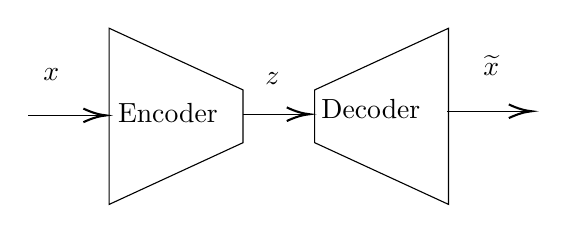
\begin{tikzpicture}[x=0.75pt,y=0.75pt,yscale=-1,xscale=1]
%uncomment if require: \path (0,300); %set diagram left start at 0, and has height of 300

%Shape: Trapezoid [id:dp8541203132727615] 
\draw   (151,77) -- (215.5,106.73) -- (215.5,132.14) -- (151,161.88) -- cycle ;
%Shape: Trapezoid [id:dp018706469204115228] 
\draw   (314.5,161.88) -- (250,132.14) -- (250,106.73) -- (314.5,77) -- cycle ;
%Straight Lines [id:da8293223382895447] 
\draw    (215.5,118.43) -- (245.5,118.43) ;
\draw [shift={(247.5,118.43)}, rotate = 180] [color={rgb, 255:red, 0; green, 0; blue, 0 }  ][line width=0.75]    (10.93,-3.29) .. controls (6.95,-1.4) and (3.31,-0.3) .. (0,0) .. controls (3.31,0.3) and (6.95,1.4) .. (10.93,3.29)   ;
%Straight Lines [id:da18164573910193638] 
\draw    (112,119) -- (147.5,119) ;
\draw [shift={(149.5,119)}, rotate = 180] [color={rgb, 255:red, 0; green, 0; blue, 0 }  ][line width=0.75]    (10.93,-3.29) .. controls (6.95,-1.4) and (3.31,-0.3) .. (0,0) .. controls (3.31,0.3) and (6.95,1.4) .. (10.93,3.29)   ;
%Straight Lines [id:da12573110589897274] 
\draw    (314,117) -- (352.5,117) ;
\draw [shift={(354.5,117)}, rotate = 180] [color={rgb, 255:red, 0; green, 0; blue, 0 }  ][line width=0.75]    (10.93,-3.29) .. controls (6.95,-1.4) and (3.31,-0.3) .. (0,0) .. controls (3.31,0.3) and (6.95,1.4) .. (10.93,3.29)   ;

% Text Node
\draw (154,112) node [anchor=north west][inner sep=0.75pt]   [align=left] {Encoder};
% Text Node
\draw (118,95) node [anchor=north west][inner sep=0.75pt]   [align=left] {$\displaystyle x$};
% Text Node
\draw (225,97) node [anchor=north west][inner sep=0.75pt]   [align=left] {$\displaystyle z$};
% Text Node
\draw (252,109.73) node [anchor=north west][inner sep=0.75pt]   [align=left] {Decoder};
% Text Node
\draw (330,89) node [anchor=north west][inner sep=0.75pt]   [align=left] {$\displaystyle \widetilde{x}$};


\end{tikzpicture}
\caption{An autoencoder}
\end{figure}

Network architecture for the Encoder and Decoder can vary wildly depending on the area of application.
In image processing it is standard practice to use 2D convolutional layers rather than fully connected dense layers.
These convolutional layers vastly reduce the number of weights needed, making training feasible in cases where a fully connected network would struggle.
They do this be reusing weights on the principle that we are interested in spacially invariant features of images, such as edges and colour gradients, rather than features localised to specific pixels.
Convolutional layers consist of many filter channels.
Each filter channel is computed by dragging a matrix of numbers known as a \textit{kernel} across the image and taking its dot product with the image at the different points.
Strictly the kernels are actually 3 dimensional matrices to account for the fact that our images and hidden cells have multiple channels.
%TODO should encoder/decoder be capitalised?

\begin{figure}[h]
  \centering
  \includegraphics[scale=0.4]{2conv.png}
  \caption{A $3 \times 3$ kernel (shaded) is convolved over a $5 \times 5$ image (lower) which has been padded with zeros to a $7 \times 7$ matrix. The resulting output is also a $5 \times 5$ matrix. (Credit: \cite{understandingConvolutions})}
\end{figure} %TODO fix this citation

A question one might be tempted to ask is what happens if we apply take the Decoder and apply it to a $z$ which has been randomly generated rather than coming via the Encoder.
We might hope that the image reconstructed by the Decoder resembles images from our original dataset.
If this were the case then we would be able to generate new images with this technique.
Unfortunately there is nothing to really guarantee this works.
If we think of our dataset as following some distribution $p(x)$ then there is not much we can say about the distribution of latent variables $p(z)$, and thus we cannot hope to directly sample a $z$ from this distribution, meaning we cannot sample a $z$ which might give a realistic $\widetilde{x}$.
Variational autoencoders are essentially designed to tackle this exact problem.

%TODO image pokemon?

\subsection{Variational Autoencoders}

Variational autoencoders \citep{kingma2013auto} consist of a convolutional Encoder and Decoder and work on a similar principle to normal autoencoders.
The encoder again takes in a high dimensional input $x$ such as an image.
However, instead of outputting a vector encoding $z$ the Encoder learns to output a distribution $q(z|x)$ of encodings representing $x$.
We require that $q(z|x)$ is a normal distribution with diagonal covariance so that the encoder actually outputs a vector twice the dimension of $z$, whose components represent the mean and covariance of $q(z|x)$.
We then sample a $z$ from this distribution and give this to the Decoder which decodes as normal to produce a reconstruction $\widetilde{x}$.
This added element of randomness is useful for reasons we will discuss shortly.

\begin{figure}[h]
  \centering


  \tikzset{every picture/.style={line width=0.75pt}} %set default line width to 0.75pt        

  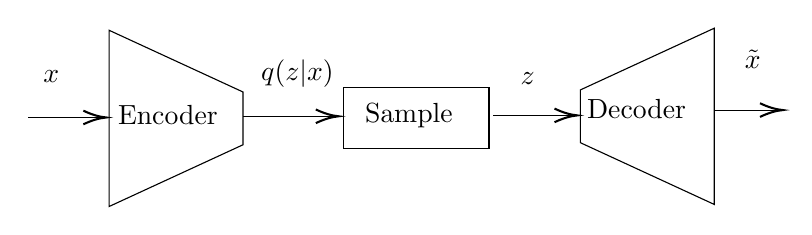
\begin{tikzpicture}[x=0.75pt,y=0.75pt,yscale=-1,xscale=1]
  %uncomment if require: \path (0,300); %set diagram left start at 0, and has height of 300
  
  %Shape: Trapezoid [id:dp8541203132727615] 
  \draw   (151,77) -- (215.5,106.73) -- (215.5,132.14) -- (151,161.88) -- cycle ;
  %Shape: Trapezoid [id:dp018706469204115228] 
  \draw   (442.5,160.88) -- (378,131.14) -- (378,105.73) -- (442.5,76) -- cycle ;
  %Straight Lines [id:da8293223382895447] 
  \draw    (215.5,118.43) -- (259.5,118.43) ;
  \draw [shift={(261.5,118.43)}, rotate = 180] [color={rgb, 255:red, 0; green, 0; blue, 0 }  ][line width=0.75]    (10.93,-3.29) .. controls (6.95,-1.4) and (3.31,-0.3) .. (0,0) .. controls (3.31,0.3) and (6.95,1.4) .. (10.93,3.29)   ;
  %Straight Lines [id:da18164573910193638] 
  \draw    (112,119) -- (147.5,119) ;
  \draw [shift={(149.5,119)}, rotate = 180] [color={rgb, 255:red, 0; green, 0; blue, 0 }  ][line width=0.75]    (10.93,-3.29) .. controls (6.95,-1.4) and (3.31,-0.3) .. (0,0) .. controls (3.31,0.3) and (6.95,1.4) .. (10.93,3.29)   ;
  %Straight Lines [id:da12573110589897274] 
  \draw    (336,118) -- (374.5,118) ;
  \draw [shift={(376.5,118)}, rotate = 180] [color={rgb, 255:red, 0; green, 0; blue, 0 }  ][line width=0.75]    (10.93,-3.29) .. controls (6.95,-1.4) and (3.31,-0.3) .. (0,0) .. controls (3.31,0.3) and (6.95,1.4) .. (10.93,3.29)   ;
  %Shape: Rectangle [id:dp9631400703948827] 
  \draw   (264,104.43) -- (334,104.43) -- (334,134) -- (264,134) -- cycle ;
  %Straight Lines [id:da9905140662945862] 
  \draw    (442.5,115.43) -- (473.5,115.43) ;
  \draw [shift={(475.5,115.43)}, rotate = 180] [color={rgb, 255:red, 0; green, 0; blue, 0 }  ][line width=0.75]    (10.93,-3.29) .. controls (6.95,-1.4) and (3.31,-0.3) .. (0,0) .. controls (3.31,0.3) and (6.95,1.4) .. (10.93,3.29)   ;
  
  % Text Node
  \draw (154,112) node [anchor=north west][inner sep=0.75pt]   [align=left] {Encoder};
  % Text Node
  \draw (118,95) node [anchor=north west][inner sep=0.75pt]   [align=left] {$\displaystyle x$};
  % Text Node
  \draw (223,90) node [anchor=north west][inner sep=0.75pt]   [align=left] {$\displaystyle q(z|x)$};
  % Text Node
  \draw (380,108.73) node [anchor=north west][inner sep=0.75pt]   [align=left] {Decoder};
  % Text Node
  \draw (456,85) node [anchor=north west][inner sep=0.75pt]   [align=left] {$\displaystyle \tilde{x}$};
  % Text Node
  \draw (273,111) node [anchor=north west][inner sep=0.75pt]   [align=left] {Sample};
  % Text Node
  \draw (348,96) node [anchor=north west][inner sep=0.75pt]   [align=left] {$\displaystyle z$};
  
  
  \end{tikzpicture}
  \caption{A variational autoencoder}
\end{figure}

We would like to train the variational autoencoder the same way we train traditional autoencoders, using backpropagation to compute the gradient of a loss function.
However, we cannot do this directly since there is no way to evaluate gradients through the random sampling process.
We get around this issue with something known as the ``reparamaterisation trick''.
Any time a datapoint is seen during training we sample an $\epsilon$ from the zero mean, unit covariance gaussian with dimension the same as $z$.
Given output vectors $\mu$ and $\sigma$ from the Encoder representing the mean and covariance of $q(z|x)$ respectively, we find that $z = \mu + \sigma \odot \epsilon$ is distributed according to $q(z|x)$.
Then for each individual datapoint we treat its sampled $\epsilon$ as a constant so that $z$ is just a function of the original input and the Encoder's weights.
This allows us to give the resulting $z$ to the Decoder and compute the gradient of the resulting loss function via backpropagation.
%one of which is that it allows us control over the distribution of latent vector 

\begin{figure}[h]
  \centering








  \tikzset{every picture/.style={line width=0.75pt}} %set default line width to 0.75pt        

  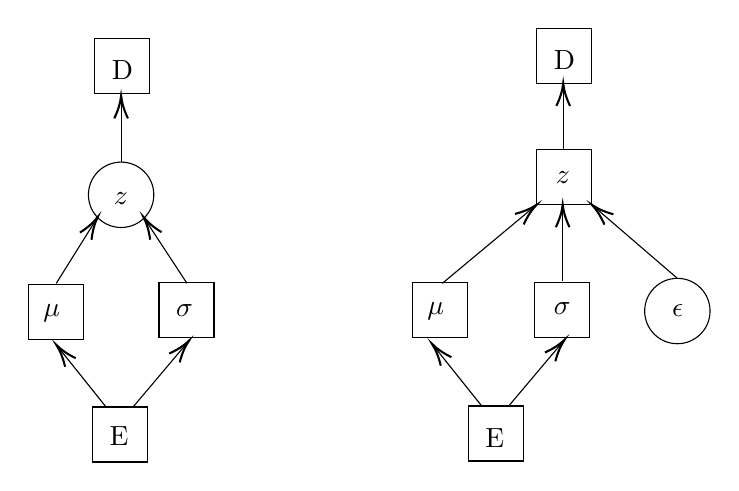
\begin{tikzpicture}[x=0.75pt,y=0.75pt,yscale=-1,xscale=1]
  %uncomment if require: \path (0,300); %set diagram left start at 0, and has height of 300
  
  %Shape: Square [id:dp31964573484955117] 
  \draw   (108,190) -- (134.5,190) -- (134.5,216.5) -- (108,216.5) -- cycle ;
  %Shape: Square [id:dp3315381522116503] 
  \draw   (171,189) -- (197.5,189) -- (197.5,215.5) -- (171,215.5) -- cycle ;
  %Shape: Circle [id:dp5157137150601787] 
  \draw   (137,146.75) .. controls (137,138.05) and (144.05,131) .. (152.75,131) .. controls (161.45,131) and (168.5,138.05) .. (168.5,146.75) .. controls (168.5,155.45) and (161.45,162.5) .. (152.75,162.5) .. controls (144.05,162.5) and (137,155.45) .. (137,146.75) -- cycle ;
  %Shape: Square [id:dp05107603102822389] 
  \draw   (293,189) -- (319.5,189) -- (319.5,215.5) -- (293,215.5) -- cycle ;
  %Shape: Square [id:dp22569528245966897] 
  \draw   (352,189) -- (378.5,189) -- (378.5,215.5) -- (352,215.5) -- cycle ;
  %Shape: Square [id:dp9307723856742833] 
  \draw   (353,125) -- (379.5,125) -- (379.5,151.5) -- (353,151.5) -- cycle ;
  %Shape: Circle [id:dp39963963544757175] 
  \draw   (405,202.75) .. controls (405,194.05) and (412.05,187) .. (420.75,187) .. controls (429.45,187) and (436.5,194.05) .. (436.5,202.75) .. controls (436.5,211.45) and (429.45,218.5) .. (420.75,218.5) .. controls (412.05,218.5) and (405,211.45) .. (405,202.75) -- cycle ;
  %Straight Lines [id:da5853904219054253] 
  \draw    (121.5,189.43) -- (140.44,159.12) ;
  \draw [shift={(141.5,157.43)}, rotate = 482.01] [color={rgb, 255:red, 0; green, 0; blue, 0 }  ][line width=0.75]    (10.93,-3.29) .. controls (6.95,-1.4) and (3.31,-0.3) .. (0,0) .. controls (3.31,0.3) and (6.95,1.4) .. (10.93,3.29)   ;
  %Straight Lines [id:da029718248550361537] 
  \draw    (184.5,189.43) -- (164.6,159.1) ;
  \draw [shift={(163.5,157.43)}, rotate = 416.73] [color={rgb, 255:red, 0; green, 0; blue, 0 }  ][line width=0.75]    (10.93,-3.29) .. controls (6.95,-1.4) and (3.31,-0.3) .. (0,0) .. controls (3.31,0.3) and (6.95,1.4) .. (10.93,3.29)   ;
  %Straight Lines [id:da21889214167912363] 
  \draw    (152.75,131) -- (152.75,101) ;
  \draw [shift={(152.75,99)}, rotate = 450] [color={rgb, 255:red, 0; green, 0; blue, 0 }  ][line width=0.75]    (10.93,-3.29) .. controls (6.95,-1.4) and (3.31,-0.3) .. (0,0) .. controls (3.31,0.3) and (6.95,1.4) .. (10.93,3.29)   ;
  %Straight Lines [id:da4460377874666688] 
  \draw    (307.5,189.43) -- (351.46,152.78) ;
  \draw [shift={(353,151.5)}, rotate = 500.19] [color={rgb, 255:red, 0; green, 0; blue, 0 }  ][line width=0.75]    (10.93,-3.29) .. controls (6.95,-1.4) and (3.31,-0.3) .. (0,0) .. controls (3.31,0.3) and (6.95,1.4) .. (10.93,3.29)   ;
  %Straight Lines [id:da6243739236469146] 
  \draw    (365.5,188.43) -- (365.5,153.43) ;
  \draw [shift={(365.5,151.43)}, rotate = 450] [color={rgb, 255:red, 0; green, 0; blue, 0 }  ][line width=0.75]    (10.93,-3.29) .. controls (6.95,-1.4) and (3.31,-0.3) .. (0,0) .. controls (3.31,0.3) and (6.95,1.4) .. (10.93,3.29)   ;
  %Straight Lines [id:da8887544337702149] 
  \draw    (420.75,187) -- (381.02,152.8) ;
  \draw [shift={(379.5,151.5)}, rotate = 400.72] [color={rgb, 255:red, 0; green, 0; blue, 0 }  ][line width=0.75]    (10.93,-3.29) .. controls (6.95,-1.4) and (3.31,-0.3) .. (0,0) .. controls (3.31,0.3) and (6.95,1.4) .. (10.93,3.29)   ;
  %Straight Lines [id:da6173989757165841] 
  \draw    (365.75,125) -- (365.75,95) ;
  \draw [shift={(365.75,93)}, rotate = 450] [color={rgb, 255:red, 0; green, 0; blue, 0 }  ][line width=0.75]    (10.93,-3.29) .. controls (6.95,-1.4) and (3.31,-0.3) .. (0,0) .. controls (3.31,0.3) and (6.95,1.4) .. (10.93,3.29)   ;
  %Shape: Square [id:dp6864470563987659] 
  \draw   (139,249) -- (165.5,249) -- (165.5,275.5) -- (139,275.5) -- cycle ;
  %Straight Lines [id:da3706413880395112] 
  \draw    (145.5,249) -- (122.75,220.56) ;
  \draw [shift={(121.5,219)}, rotate = 411.34000000000003] [color={rgb, 255:red, 0; green, 0; blue, 0 }  ][line width=0.75]    (10.93,-3.29) .. controls (6.95,-1.4) and (3.31,-0.3) .. (0,0) .. controls (3.31,0.3) and (6.95,1.4) .. (10.93,3.29)   ;
  %Straight Lines [id:da15484413544209885] 
  \draw    (158.5,249) -- (184.21,218.53) ;
  \draw [shift={(185.5,217)}, rotate = 490.16] [color={rgb, 255:red, 0; green, 0; blue, 0 }  ][line width=0.75]    (10.93,-3.29) .. controls (6.95,-1.4) and (3.31,-0.3) .. (0,0) .. controls (3.31,0.3) and (6.95,1.4) .. (10.93,3.29)   ;
  %Shape: Square [id:dp9985017530467823] 
  \draw   (320,248.5) -- (346.5,248.5) -- (346.5,275) -- (320,275) -- cycle ;
  %Straight Lines [id:da003142022678509937] 
  \draw    (326.5,248.5) -- (303.75,220.06) ;
  \draw [shift={(302.5,218.5)}, rotate = 411.34000000000003] [color={rgb, 255:red, 0; green, 0; blue, 0 }  ][line width=0.75]    (10.93,-3.29) .. controls (6.95,-1.4) and (3.31,-0.3) .. (0,0) .. controls (3.31,0.3) and (6.95,1.4) .. (10.93,3.29)   ;
  %Straight Lines [id:da2704203996875034] 
  \draw    (339.5,248.5) -- (365.21,218.03) ;
  \draw [shift={(366.5,216.5)}, rotate = 490.16] [color={rgb, 255:red, 0; green, 0; blue, 0 }  ][line width=0.75]    (10.93,-3.29) .. controls (6.95,-1.4) and (3.31,-0.3) .. (0,0) .. controls (3.31,0.3) and (6.95,1.4) .. (10.93,3.29)   ;
  %Shape: Square [id:dp7340240930655411] 
  \draw   (353,66.5) -- (379.5,66.5) -- (379.5,93) -- (353,93) -- cycle ;
  %Shape: Square [id:dp21421435030738412] 
  \draw   (140,71.5) -- (166.5,71.5) -- (166.5,98) -- (140,98) -- cycle ;
  
  % Text Node
  \draw (114,198.4) node [anchor=north west][inner sep=0.75pt]    {$\mu $};
  % Text Node
  \draw (178,198.4) node [anchor=north west][inner sep=0.75pt]    {$\sigma $};
  % Text Node
  \draw (148,144.4) node [anchor=north west][inner sep=0.75pt]    {$z$};
  % Text Node
  \draw (299,197.4) node [anchor=north west][inner sep=0.75pt]    {$\mu $};
  % Text Node
  \draw (360,197.4) node [anchor=north west][inner sep=0.75pt]    {$\sigma $};
  % Text Node
  \draw (361,134.4) node [anchor=north west][inner sep=0.75pt]    {$z$};
  % Text Node
  \draw (417,198.4) node [anchor=north west][inner sep=0.75pt]    {$\epsilon $};
  % Text Node
  \draw (146,257) node [anchor=north west][inner sep=0.75pt]   [align=left] {E};
  % Text Node
  \draw (327,258) node [anchor=north west][inner sep=0.75pt]   [align=left] {E};
  % Text Node
  \draw (360,76) node [anchor=north west][inner sep=0.75pt]   [align=left] {D};
  % Text Node
  \draw (147,81) node [anchor=north west][inner sep=0.75pt]   [align=left] {D};
  
  
  \end{tikzpicture}
\caption{Removing the gradient-blocking stochastic node with the reparamaterisation trick.}
\end{figure}

If we used the same loss function as a traditional autoencoder then the network would simply learn to reduce the covariance of $q(z|x)$ in order to reduce noise in its latent representations.
Thus we introduce a term to the loss function which constrains the form of $q(z|x)$.
Ultimately we are interested in being able to sample realistic latent variables from the ``true distribution'' $p(z)$, and we make the arbitrary choice that we want to be able to do this simply by sampling from the zero mean unit covariance normal distribution, so we penalise $q(z|x)$ the further from this distribution it is.
We do this using a measure of similarity of probability distributions known as the KL divergence of the two distributions.
In this case it can be computed in closed form as
$$D_{KL}(q(z|x),p(z)) = \sum_{i=1}^d \sigma_i^2 + \mu_i^2 - \log(\sigma_i)-1$$
There is a more formal probabilistic justification of the use of KL-divergence here that also suggests the use of a cross entropy reconstruction loss.
Since World Models uses a least squares loss rather than the more probabilistic approach we won't discuss this interpretation further, but for the interested more details can be found in the original paper \citep{kingma2013auto}.


\section{Memory}
The Memory component $M$ of World Models forms the bulk of the agent's internal model.
It is trained to learn the probability distribution $p(z_{t+1} | z_t, a_t, h_t)$ which when combined with the Vision component can be used to produce interactive dreams of the agent's environment.
$M$ consists of a neural network known as a Mixture Density Reccurrent Neural Network (MDRNN).
This has two components: the input LSTM layer which provides the memory functionality and the output Mixture Density layer which allows the network to output a probability distribution.
Similarly to the last section this section gives a somewhat broad description of MDRNNs, and World Models specific implementation details can be found in \ref{MDRNNsubsec}.

\begin{figure}[h]
  \centering


\tikzset{every picture/.style={line width=0.75pt}} %set default line width to 0.75pt        

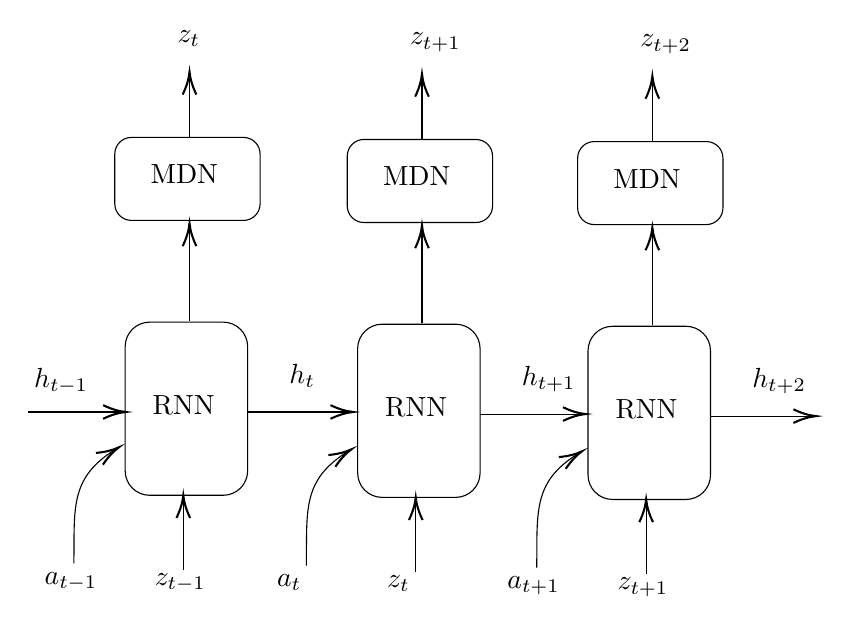
\begin{tikzpicture}[x=0.75pt,y=0.75pt,yscale=-1,xscale=1]
%uncomment if require: \path (0,363); %set diagram left start at 0, and has height of 363

%Rounded Rect [id:dp7430947240092758] 
\draw   (153.07,174.8) .. controls (153.07,168.28) and (158.35,163) .. (164.87,163) -- (200.27,163) .. controls (206.79,163) and (212.07,168.28) .. (212.07,174.8) -- (212.07,234.63) .. controls (212.07,241.15) and (206.79,246.43) .. (200.27,246.43) -- (164.87,246.43) .. controls (158.35,246.43) and (153.07,241.15) .. (153.07,234.63) -- cycle ;
%Rounded Rect [id:dp7429822235575114] 
\draw   (148.07,82) .. controls (148.07,77.58) and (151.65,74) .. (156.07,74) -- (210.07,74) .. controls (214.49,74) and (218.07,77.58) .. (218.07,82) -- (218.07,106) .. controls (218.07,110.42) and (214.49,114) .. (210.07,114) -- (156.07,114) .. controls (151.65,114) and (148.07,110.42) .. (148.07,106) -- cycle ;
%Straight Lines [id:da7494592707832595] 
\draw    (184.07,74.43) -- (184.07,44.43) ;
\draw [shift={(184.07,42.43)}, rotate = 450] [color={rgb, 255:red, 0; green, 0; blue, 0 }  ][line width=0.75]    (10.93,-3.29) .. controls (6.95,-1.4) and (3.31,-0.3) .. (0,0) .. controls (3.31,0.3) and (6.95,1.4) .. (10.93,3.29)   ;
%Straight Lines [id:da7228370640214785] 
\draw    (184.07,162.43) -- (184.07,117.43) ;
\draw [shift={(184.07,115.43)}, rotate = 450] [color={rgb, 255:red, 0; green, 0; blue, 0 }  ][line width=0.75]    (10.93,-3.29) .. controls (6.95,-1.4) and (3.31,-0.3) .. (0,0) .. controls (3.31,0.3) and (6.95,1.4) .. (10.93,3.29)   ;
%Straight Lines [id:da8085002894425344] 
\draw    (181.07,282.43) -- (181.07,248.43) ;
\draw [shift={(181.07,246.43)}, rotate = 450] [color={rgb, 255:red, 0; green, 0; blue, 0 }  ][line width=0.75]    (10.93,-3.29) .. controls (6.95,-1.4) and (3.31,-0.3) .. (0,0) .. controls (3.31,0.3) and (6.95,1.4) .. (10.93,3.29)   ;
%Curve Lines [id:da9147039112573743] 
\draw    (128.36,279.29) .. controls (128.64,251.85) and (126.45,237.85) .. (148.68,224.13) ;
\draw [shift={(150.07,223.29)}, rotate = 509.44] [color={rgb, 255:red, 0; green, 0; blue, 0 }  ][line width=0.75]    (10.93,-3.29) .. controls (6.95,-1.4) and (3.31,-0.3) .. (0,0) .. controls (3.31,0.3) and (6.95,1.4) .. (10.93,3.29)   ;
%Straight Lines [id:da4978899346146559] 
\draw    (211.93,206.29) -- (260.93,206.29) ;
\draw [shift={(262.93,206.29)}, rotate = 180] [color={rgb, 255:red, 0; green, 0; blue, 0 }  ][line width=0.75]    (10.93,-3.29) .. controls (6.95,-1.4) and (3.31,-0.3) .. (0,0) .. controls (3.31,0.3) and (6.95,1.4) .. (10.93,3.29)   ;
%Rounded Rect [id:dp21684587264636557] 
\draw   (265.07,175.8) .. controls (265.07,169.28) and (270.35,164) .. (276.87,164) -- (312.27,164) .. controls (318.79,164) and (324.07,169.28) .. (324.07,175.8) -- (324.07,235.63) .. controls (324.07,242.15) and (318.79,247.43) .. (312.27,247.43) -- (276.87,247.43) .. controls (270.35,247.43) and (265.07,242.15) .. (265.07,235.63) -- cycle ;
%Rounded Rect [id:dp574116066843422] 
\draw   (260.07,83) .. controls (260.07,78.58) and (263.65,75) .. (268.07,75) -- (322.07,75) .. controls (326.49,75) and (330.07,78.58) .. (330.07,83) -- (330.07,107) .. controls (330.07,111.42) and (326.49,115) .. (322.07,115) -- (268.07,115) .. controls (263.65,115) and (260.07,111.42) .. (260.07,107) -- cycle ;
%Straight Lines [id:da13341755017886814] 
\draw    (296.07,75.43) -- (296.07,45.43) ;
\draw [shift={(296.07,43.43)}, rotate = 450] [color={rgb, 255:red, 0; green, 0; blue, 0 }  ][line width=0.75]    (10.93,-3.29) .. controls (6.95,-1.4) and (3.31,-0.3) .. (0,0) .. controls (3.31,0.3) and (6.95,1.4) .. (10.93,3.29)   ;
%Straight Lines [id:da6061008181274479] 
\draw    (296.07,163.43) -- (296.07,118.43) ;
\draw [shift={(296.07,116.43)}, rotate = 450] [color={rgb, 255:red, 0; green, 0; blue, 0 }  ][line width=0.75]    (10.93,-3.29) .. controls (6.95,-1.4) and (3.31,-0.3) .. (0,0) .. controls (3.31,0.3) and (6.95,1.4) .. (10.93,3.29)   ;
%Straight Lines [id:da7962048588570034] 
\draw    (293.07,283.43) -- (293.07,249.43) ;
\draw [shift={(293.07,247.43)}, rotate = 450] [color={rgb, 255:red, 0; green, 0; blue, 0 }  ][line width=0.75]    (10.93,-3.29) .. controls (6.95,-1.4) and (3.31,-0.3) .. (0,0) .. controls (3.31,0.3) and (6.95,1.4) .. (10.93,3.29)   ;
%Curve Lines [id:da06723740780427412] 
\draw    (240.36,280.29) .. controls (240.64,252.85) and (238.45,238.85) .. (260.68,225.13) ;
\draw [shift={(262.07,224.29)}, rotate = 509.44] [color={rgb, 255:red, 0; green, 0; blue, 0 }  ][line width=0.75]    (10.93,-3.29) .. controls (6.95,-1.4) and (3.31,-0.3) .. (0,0) .. controls (3.31,0.3) and (6.95,1.4) .. (10.93,3.29)   ;
%Straight Lines [id:da026804072896316145] 
\draw    (323.93,207.29) -- (372.93,207.29) ;
\draw [shift={(374.93,207.29)}, rotate = 180] [color={rgb, 255:red, 0; green, 0; blue, 0 }  ][line width=0.75]    (10.93,-3.29) .. controls (6.95,-1.4) and (3.31,-0.3) .. (0,0) .. controls (3.31,0.3) and (6.95,1.4) .. (10.93,3.29)   ;
%Rounded Rect [id:dp5485476783727927] 
\draw   (376.07,176.8) .. controls (376.07,170.28) and (381.35,165) .. (387.87,165) -- (423.27,165) .. controls (429.79,165) and (435.07,170.28) .. (435.07,176.8) -- (435.07,236.63) .. controls (435.07,243.15) and (429.79,248.43) .. (423.27,248.43) -- (387.87,248.43) .. controls (381.35,248.43) and (376.07,243.15) .. (376.07,236.63) -- cycle ;
%Rounded Rect [id:dp9766477067537895] 
\draw   (371.07,84) .. controls (371.07,79.58) and (374.65,76) .. (379.07,76) -- (433.07,76) .. controls (437.49,76) and (441.07,79.58) .. (441.07,84) -- (441.07,108) .. controls (441.07,112.42) and (437.49,116) .. (433.07,116) -- (379.07,116) .. controls (374.65,116) and (371.07,112.42) .. (371.07,108) -- cycle ;
%Straight Lines [id:da15122846554522162] 
\draw    (407.07,76.43) -- (407.07,46.43) ;
\draw [shift={(407.07,44.43)}, rotate = 450] [color={rgb, 255:red, 0; green, 0; blue, 0 }  ][line width=0.75]    (10.93,-3.29) .. controls (6.95,-1.4) and (3.31,-0.3) .. (0,0) .. controls (3.31,0.3) and (6.95,1.4) .. (10.93,3.29)   ;
%Straight Lines [id:da12481781992958196] 
\draw    (407.07,164.43) -- (407.07,119.43) ;
\draw [shift={(407.07,117.43)}, rotate = 450] [color={rgb, 255:red, 0; green, 0; blue, 0 }  ][line width=0.75]    (10.93,-3.29) .. controls (6.95,-1.4) and (3.31,-0.3) .. (0,0) .. controls (3.31,0.3) and (6.95,1.4) .. (10.93,3.29)   ;
%Straight Lines [id:da1600245319817022] 
\draw    (404.07,284.43) -- (404.07,250.43) ;
\draw [shift={(404.07,248.43)}, rotate = 450] [color={rgb, 255:red, 0; green, 0; blue, 0 }  ][line width=0.75]    (10.93,-3.29) .. controls (6.95,-1.4) and (3.31,-0.3) .. (0,0) .. controls (3.31,0.3) and (6.95,1.4) .. (10.93,3.29)   ;
%Curve Lines [id:da6377994512542458] 
\draw    (351.36,281.29) .. controls (351.64,253.85) and (349.45,239.85) .. (371.68,226.13) ;
\draw [shift={(373.07,225.29)}, rotate = 509.44] [color={rgb, 255:red, 0; green, 0; blue, 0 }  ][line width=0.75]    (10.93,-3.29) .. controls (6.95,-1.4) and (3.31,-0.3) .. (0,0) .. controls (3.31,0.3) and (6.95,1.4) .. (10.93,3.29)   ;
%Straight Lines [id:da9236269480372257] 
\draw    (434.93,208.29) -- (483.93,208.29) ;
\draw [shift={(485.93,208.29)}, rotate = 180] [color={rgb, 255:red, 0; green, 0; blue, 0 }  ][line width=0.75]    (10.93,-3.29) .. controls (6.95,-1.4) and (3.31,-0.3) .. (0,0) .. controls (3.31,0.3) and (6.95,1.4) .. (10.93,3.29)   ;
%Straight Lines [id:da6161697921472136] 
\draw    (106.36,206.29) -- (151.36,206.29) ;
\draw [shift={(153.36,206.29)}, rotate = 180] [color={rgb, 255:red, 0; green, 0; blue, 0 }  ][line width=0.75]    (10.93,-3.29) .. controls (6.95,-1.4) and (3.31,-0.3) .. (0,0) .. controls (3.31,0.3) and (6.95,1.4) .. (10.93,3.29)   ;

% Text Node
\draw (165.07,197) node [anchor=north west][inner sep=0.75pt]   [align=left] {RNN};
% Text Node
\draw (164.07,86) node [anchor=north west][inner sep=0.75pt]   [align=left] {MDN};
% Text Node
\draw (177.07,21.4) node [anchor=north west][inner sep=0.75pt]    {$z_{t}$};
% Text Node
\draw (166.07,283) node [anchor=north west][inner sep=0.75pt]   [align=left] {$\displaystyle z_{t-1}$};
% Text Node
\draw (113,282.4) node [anchor=north west][inner sep=0.75pt]    {$a_{t-1}$};
% Text Node
\draw (230.93,182) node [anchor=north west][inner sep=0.75pt]   [align=left] {$\displaystyle h_{t}$};
% Text Node
\draw (277.07,198) node [anchor=north west][inner sep=0.75pt]   [align=left] {RNN};
% Text Node
\draw (276.07,87) node [anchor=north west][inner sep=0.75pt]   [align=left] {MDN};
% Text Node
\draw (289.07,22.4) node [anchor=north west][inner sep=0.75pt]    {$z_{t+1}$};
% Text Node
\draw (278.07,284) node [anchor=north west][inner sep=0.75pt]   [align=left] {$\displaystyle z_{t}$};
% Text Node
\draw (225,283.4) node [anchor=north west][inner sep=0.75pt]    {$a_{t}$};
% Text Node
\draw (342.93,183) node [anchor=north west][inner sep=0.75pt]   [align=left] {$\displaystyle h_{t+1}$};
% Text Node
\draw (388.07,199) node [anchor=north west][inner sep=0.75pt]   [align=left] {RNN};
% Text Node
\draw (387.07,88) node [anchor=north west][inner sep=0.75pt]   [align=left] {MDN};
% Text Node
\draw (400.07,23.4) node [anchor=north west][inner sep=0.75pt]    {$z_{t+2}$};
% Text Node
\draw (389.07,285) node [anchor=north west][inner sep=0.75pt]   [align=left] {$\displaystyle z_{t+1}$};
% Text Node
\draw (336,284.4) node [anchor=north west][inner sep=0.75pt]    {$a_{t+1}$};
% Text Node
\draw (453.93,184) node [anchor=north west][inner sep=0.75pt]   [align=left] {$\displaystyle h_{t+2}$};
% Text Node
\draw (107.93,184) node [anchor=north west][inner sep=0.75pt]   [align=left] {$\displaystyle h_{t-1}$};


\end{tikzpicture}
\caption{The Memory component combines an RNN and MDN to predict the distribution of the next latent variable $z$.}
\label{memFig}
\end{figure}

\subsection{Long Short Term Memory}
Recurrent neural nets (RNNs) are common in problems where data is sequential, for example text, audio or video data.
RNNs are composed of one or more reccurrent layers.
In addition to taking an element of the sequence (like a  word, note, or image) as their input these recurrent layers are also given their own output on the previous element of the sequence.
Since this output in turn depends on the output of the layer on the element before that (and so on) the result is a sequential reccurence as depicted in Figure \ref{memFig}.
RNNs are trained by gradient descent by evaluating the \textit{unrolled} network's output on an entire sequence and using backpropagation to propagate gradients both vertically through the network and horizontally through time.

Classical fully connected RNNs often suffer from what is known as the \textit{vanishing gradient problem} \citep{hochreiter1991untersuchungen}.
Essentially, the chain rule means the backpropgation is multiplicative across the recurrent connections and thus gradient information decays (or explodes) exponentially with the distance in the sequence, making it hard for classical RNNs to learn to maintain long term memory. 
Long Short Term Memory Networks (LSTMs) are designed to address this problem.
They do this by maintaining separate protected memory cells $c$ which can only be changed or read by the network through a series of gates, ensuring that gradient contributions remain constant over time.
At a timestep $t$ an LSTM layer reads in input $x_t$, as well as its own previous cell value $c_{t-1}$ and previous output $h_{t-1}$.
It computes both new cell values $c_t$ and output $h_t$, however the network at that time step is only given $h_t$ and does not directly see $c_t$.
At each timestep the memory cells go through three gates, each with its own learned weights.
The first gate is the forget gate, where the cell values are multiplied componentwise by $\sigma( W_f\cdot [h_{t-1},x_t]+b_f)$.
Here $W_f$ and $b_f$ are learned weights and the sigmoid activation results in outputs between 0 and 1, so that values closer to 0 cause the corresponding cell to be forgotten and values closer to 1 cause it to be remembered.
The second gate is the input gate.
New information to be added to the cells is calculated as $\tanh( W_c\cdot [h_{t-1},x_t]+b_c)$.
Another sigmoid activation $\sigma( W_i\cdot [h_{t-1},x_t]+b_i)$ is multiplied with this information to decide what should be accepted and the result is added to the cell values to form $c_t$.
Finally the output gate scales $\tanh(c_t)$ by $\sigma( W_o\cdot [h_{t-1},x_t]+b_o)$ to determine the output $h_t$.


\begin{figure}[h]
  \centering






  \tikzset{every picture/.style={line width=0.75pt}} %set default line width to 0.75pt        

  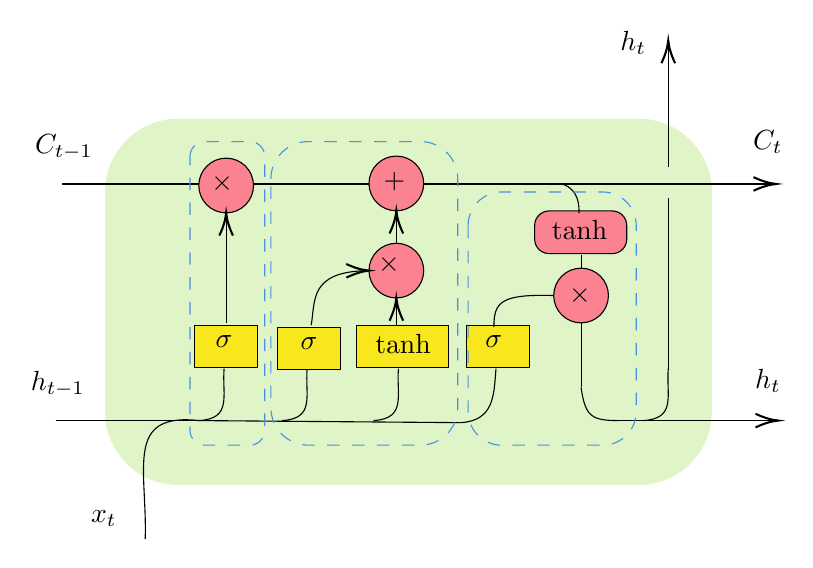
\begin{tikzpicture}[x=0.75pt,y=0.75pt,yscale=-1,xscale=1]
  %uncomment if require: \path (0,300); %set diagram left start at 0, and has height of 300
  
  %Rounded Rect [id:dp7644481375883001] 
  \draw  [draw opacity=0][fill={rgb, 255:red, 126; green, 211; blue, 33 }  ,fill opacity=0.25 ] (66,92.29) .. controls (66,72.8) and (81.8,57) .. (101.29,57) -- (323.07,57) .. controls (342.56,57) and (358.36,72.8) .. (358.36,92.29) -- (358.36,198.14) .. controls (358.36,217.63) and (342.56,233.43) .. (323.07,233.43) -- (101.29,233.43) .. controls (81.8,233.43) and (66,217.63) .. (66,198.14) -- cycle ;
  %Straight Lines [id:da14977972949454688] 
  \draw    (45.36,88.43) -- (387.36,88.43) ;
  \draw [shift={(389.36,88.43)}, rotate = 180] [color={rgb, 255:red, 0; green, 0; blue, 0 }  ][line width=0.75]    (10.93,-3.29) .. controls (6.95,-1.4) and (3.31,-0.3) .. (0,0) .. controls (3.31,0.3) and (6.95,1.4) .. (10.93,3.29)   ;
  %Curve Lines [id:da36560052384334196] 
  \draw    (85.36,259.43) .. controls (86.36,225.43) and (75.36,198.43) .. (111.36,202.43) ;
  %Straight Lines [id:da5858359446293169] 
  \draw    (42.36,202.43) -- (111.36,202.43) ;
  %Curve Lines [id:da9040025231719764] 
  \draw    (111.36,202.43) .. controls (127.36,201.43) and (122.36,190.43) .. (123.36,177.43) ;
  %Shape: Rectangle [id:dp5386952386344248] 
  \draw  [fill={rgb, 255:red, 248; green, 231; blue, 28 }  ,fill opacity=1 ] (109,156.43) -- (139.36,156.43) -- (139.36,177) -- (109,177) -- cycle ;
  %Shape: Circle [id:dp24827607695419052] 
  \draw  [fill={rgb, 255:red, 250; green, 130; blue, 145 }  ,fill opacity=1 ] (111.18,89.18) .. controls (111.18,81.9) and (117.08,76) .. (124.36,76) .. controls (131.64,76) and (137.54,81.9) .. (137.54,89.18) .. controls (137.54,96.46) and (131.64,102.36) .. (124.36,102.36) .. controls (117.08,102.36) and (111.18,96.46) .. (111.18,89.18) -- cycle ;
  %Straight Lines [id:da9219708528408646] 
  \draw    (124.36,155.43) -- (124.36,104.36) ;
  \draw [shift={(124.36,102.36)}, rotate = 450] [color={rgb, 255:red, 0; green, 0; blue, 0 }  ][line width=0.75]    (10.93,-3.29) .. controls (6.95,-1.4) and (3.31,-0.3) .. (0,0) .. controls (3.31,0.3) and (6.95,1.4) .. (10.93,3.29)   ;
  %Straight Lines [id:da47393213977371973] 
  \draw    (111.36,202.43) -- (237.36,203.43) ;
  %Curve Lines [id:da9206419555540606] 
  \draw    (151.36,202.43) .. controls (167.36,201.43) and (162.36,190.43) .. (163.36,177.43) ;
  %Curve Lines [id:da7582972370990808] 
  \draw    (195.36,202.43) .. controls (211.36,201.43) and (206.36,190.43) .. (207.36,177.43) ;
  %Shape: Rectangle [id:dp2198207899620419] 
  \draw  [fill={rgb, 255:red, 248; green, 231; blue, 28 }  ,fill opacity=1 ] (149,157.43) -- (179.36,157.43) -- (179.36,178) -- (149,178) -- cycle ;
  %Shape: Rectangle [id:dp16233653855602004] 
  \draw  [fill={rgb, 255:red, 248; green, 231; blue, 28 }  ,fill opacity=1 ] (187,156.43) -- (231.36,156.43) -- (231.36,177) -- (187,177) -- cycle ;
  %Shape: Circle [id:dp00028065792295373093] 
  \draw  [fill={rgb, 255:red, 250; green, 130; blue, 145 }  ,fill opacity=1 ] (193.18,130.18) .. controls (193.18,122.9) and (199.08,117) .. (206.36,117) .. controls (213.64,117) and (219.54,122.9) .. (219.54,130.18) .. controls (219.54,137.46) and (213.64,143.36) .. (206.36,143.36) .. controls (199.08,143.36) and (193.18,137.46) .. (193.18,130.18) -- cycle ;
  %Shape: Circle [id:dp35773285784240216] 
  \draw  [fill={rgb, 255:red, 250; green, 130; blue, 145 }  ,fill opacity=1 ] (193.18,88.18) .. controls (193.18,80.9) and (199.08,75) .. (206.36,75) .. controls (213.64,75) and (219.54,80.9) .. (219.54,88.18) .. controls (219.54,95.46) and (213.64,101.36) .. (206.36,101.36) .. controls (199.08,101.36) and (193.18,95.46) .. (193.18,88.18) -- cycle ;
  %Shape: Circle [id:dp9984490333965701] 
  \draw  [fill={rgb, 255:red, 250; green, 130; blue, 145 }  ,fill opacity=1 ] (282.18,142.18) .. controls (282.18,134.9) and (288.08,129) .. (295.36,129) .. controls (302.64,129) and (308.54,134.9) .. (308.54,142.18) .. controls (308.54,149.46) and (302.64,155.36) .. (295.36,155.36) .. controls (288.08,155.36) and (282.18,149.46) .. (282.18,142.18) -- cycle ;
  %Curve Lines [id:da4297917696834421] 
  \draw    (165.36,156.43) .. controls (167.32,144.67) and (164.48,130.99) .. (191.49,130.21) ;
  \draw [shift={(193.18,130.18)}, rotate = 539.5] [color={rgb, 255:red, 0; green, 0; blue, 0 }  ][line width=0.75]    (10.93,-3.29) .. controls (6.95,-1.4) and (3.31,-0.3) .. (0,0) .. controls (3.31,0.3) and (6.95,1.4) .. (10.93,3.29)   ;
  %Straight Lines [id:da6262632387476696] 
  \draw    (206.36,156.43) -- (206.36,145.36) ;
  \draw [shift={(206.36,143.36)}, rotate = 450] [color={rgb, 255:red, 0; green, 0; blue, 0 }  ][line width=0.75]    (10.93,-3.29) .. controls (6.95,-1.4) and (3.31,-0.3) .. (0,0) .. controls (3.31,0.3) and (6.95,1.4) .. (10.93,3.29)   ;
  %Straight Lines [id:da6429279191222157] 
  \draw    (206.36,117) -- (206.36,103.36) ;
  \draw [shift={(206.36,101.36)}, rotate = 450] [color={rgb, 255:red, 0; green, 0; blue, 0 }  ][line width=0.75]    (10.93,-3.29) .. controls (6.95,-1.4) and (3.31,-0.3) .. (0,0) .. controls (3.31,0.3) and (6.95,1.4) .. (10.93,3.29)   ;
  %Shape: Rectangle [id:dp6426648146347886] 
  \draw  [fill={rgb, 255:red, 248; green, 231; blue, 28 }  ,fill opacity=1 ] (240,156.43) -- (270.36,156.43) -- (270.36,177) -- (240,177) -- cycle ;
  %Curve Lines [id:da6718405121494726] 
  \draw    (237.36,203.43) .. controls (253.36,202.43) and (253.36,190.43) .. (254.36,177.43) ;
  %Curve Lines [id:da05718705579556116] 
  \draw    (253.36,157.43) .. controls (253.36,145.43) and (256.36,141.43) .. (282.18,142.18) ;
  %Shape: Rectangle [id:dp5785920877058888] 
  \draw  [fill={rgb, 255:red, 250; green, 130; blue, 145 }  ,fill opacity=1 ] (273,108.43) .. controls (273,104.56) and (276.13,101.43) .. (280,101.43) -- (310.36,101.43) .. controls (314.22,101.43) and (317.36,104.56) .. (317.36,108.43) -- (317.36,115) .. controls (317.36,118.87) and (314.22,122) .. (310.36,122) -- (280,122) .. controls (276.13,122) and (273,118.87) .. (273,115) -- cycle ;
  %Curve Lines [id:da6810023243615051] 
  \draw    (286.36,88.43) .. controls (294.36,91.43) and (294.36,98.43) .. (294.36,102.43) ;
  %Straight Lines [id:da1328492474823424] 
  \draw    (295.36,129) -- (295.36,122.43) ;
  %Straight Lines [id:da6932574999115595] 
  \draw    (313.36,202.43) -- (388.36,202.43) ;
  \draw [shift={(390.36,202.43)}, rotate = 180] [color={rgb, 255:red, 0; green, 0; blue, 0 }  ][line width=0.75]    (10.93,-3.29) .. controls (6.95,-1.4) and (3.31,-0.3) .. (0,0) .. controls (3.31,0.3) and (6.95,1.4) .. (10.93,3.29)   ;
  %Straight Lines [id:da09230780170649977] 
  \draw    (295.36,155.36) -- (295.36,186.43) ;
  %Curve Lines [id:da8312301392191521] 
  \draw    (295.36,186.43) .. controls (297.36,200.43) and (300.36,202.43) .. (313.36,202.43) ;
  %Curve Lines [id:da9758555031264495] 
  \draw    (325.36,202.43) .. controls (341.36,201.43) and (336.36,190.43) .. (337.36,177.43) ;
  %Straight Lines [id:da3635538651240182] 
  \draw    (337.36,177.43) -- (337.36,95.29) ;
  %Straight Lines [id:da6966096252928047] 
  \draw    (337.36,80.29) -- (337.36,21.29) ;
  \draw [shift={(337.36,19.29)}, rotate = 450] [color={rgb, 255:red, 0; green, 0; blue, 0 }  ][line width=0.75]    (10.93,-3.29) .. controls (6.95,-1.4) and (3.31,-0.3) .. (0,0) .. controls (3.31,0.3) and (6.95,1.4) .. (10.93,3.29)   ;
  %Rounded Rect [id:dp06773438982764102] 
  \draw  [color={rgb, 255:red, 74; green, 144; blue, 226 }  ,draw opacity=1 ][dash pattern={on 4.5pt off 4.5pt}] (106.93,75.2) .. controls (106.93,71.22) and (110.15,68) .. (114.13,68) -- (135.73,68) .. controls (139.71,68) and (142.93,71.22) .. (142.93,75.2) -- (142.93,207.09) .. controls (142.93,211.06) and (139.71,214.29) .. (135.73,214.29) -- (114.13,214.29) .. controls (110.15,214.29) and (106.93,211.06) .. (106.93,207.09) -- cycle ;
  %Rounded Rect [id:dp366292533696718] 
  \draw  [color={rgb, 255:red, 74; green, 144; blue, 226 }  ,draw opacity=1 ][dash pattern={on 4.5pt off 4.5pt}] (145.93,86) .. controls (145.93,76.06) and (153.99,68) .. (163.93,68) -- (217.93,68) .. controls (227.87,68) and (235.93,76.06) .. (235.93,86) -- (235.93,196.29) .. controls (235.93,206.23) and (227.87,214.29) .. (217.93,214.29) -- (163.93,214.29) .. controls (153.99,214.29) and (145.93,206.23) .. (145.93,196.29) -- cycle ;
  %Rounded Rect [id:dp859119350521788] 
  \draw  [color={rgb, 255:red, 74; green, 144; blue, 226 }  ,draw opacity=1 ][dash pattern={on 4.5pt off 4.5pt}] (240.93,108.49) .. controls (240.93,99.54) and (248.18,92.29) .. (257.13,92.29) -- (305.73,92.29) .. controls (314.68,92.29) and (321.93,99.54) .. (321.93,108.49) -- (321.93,198.09) .. controls (321.93,207.03) and (314.68,214.29) .. (305.73,214.29) -- (257.13,214.29) .. controls (248.18,214.29) and (240.93,207.03) .. (240.93,198.09) -- cycle ;
  
  % Text Node
  \draw (31,63.4) node [anchor=north west][inner sep=0.75pt]    {$C_{t-1}$};
  % Text Node
  \draw (377,61.4) node [anchor=north west][inner sep=0.75pt]    {$C_{t}$};
  % Text Node
  \draw (58,244.4) node [anchor=north west][inner sep=0.75pt]    {$x_{t}$};
  % Text Node
  \draw (29,177.4) node [anchor=north west][inner sep=0.75pt]    {$h_{t-1}$};
  % Text Node
  \draw (378,176.4) node [anchor=north west][inner sep=0.75pt]    {$h_{t}$};
  % Text Node
  \draw (118,160) node [anchor=north west][inner sep=0.75pt]   [align=left] {$\displaystyle \sigma $};
  % Text Node
  \draw (116,82.4) node [anchor=north west][inner sep=0.75pt]    {$\times $};
  % Text Node
  \draw (159,161) node [anchor=north west][inner sep=0.75pt]   [align=left] {$\displaystyle \sigma $};
  % Text Node
  \draw (195,159.43) node [anchor=north west][inner sep=0.75pt]   [align=left] {tanh};
  % Text Node
  \draw (196.36,121.4) node [anchor=north west][inner sep=0.75pt]    {$\times $};
  % Text Node
  \draw (199,81.4) node [anchor=north west][inner sep=0.75pt]    {$+$};
  % Text Node
  \draw (248,160) node [anchor=north west][inner sep=0.75pt]   [align=left] {$\displaystyle \sigma $};
  % Text Node
  \draw (280,104.43) node [anchor=north west][inner sep=0.75pt]   [align=left] {tanh};
  % Text Node
  \draw (288.36,136.4) node [anchor=north west][inner sep=0.75pt]    {$\times $};
  % Text Node
  \draw (313,13.4) node [anchor=north west][inner sep=0.75pt]    {$h_{t}$};
  
  
  \end{tikzpicture}
\caption{An LSTM layer. The forget, input, and output gates are outlined in blue from left to right. (Credit: \cite{understandingLSTM}) }
\end{figure}
\subsection{Mixture Density Nets}
A mixture density net (MDN) is a type of feedforward neural net, categorised by its output layer and loss function, that learns probability distributions.
That is, given an input vector $x$, rather than returning a prediction $z$ an MDN returns a distribution of predictions $p(z|x)$.
This is useful for learning to fit data where an input $x$ might correspond to a wide range of target $z$, for example data coming from multivalued functions.
The idea is in principle similar to the encoder in a VAE in that we restrict our attention to a parameterised family of distributions and the neural network learns to output these parameters.
The family we choose is what is known as a \textit{mixture distribution} and consists of a weighted sum or ``mixture'' of a fixed number $K$ of parameterised distributions (``mixture components'').
Most commonly (and in World Models) mixture components are Gaussians with diagonal covariance matrices, thus the MDN learns a distribution
$$p(z|x) = \sum_{k=1}^K \pi_k \mathcal{N}\left(z|\mu_k, \Sigma_k\right)$$
with mixture weights $\pi_k$, means $\mu_k$ and covariances $\Sigma_k$ as its output.
Note that we must have $\sum_{k=1}^K \pi_k = 1$ for this distribution to correctly integrate to one.

% \begin{figure}[h]
%   \centering

%   \caption{A Gaussian Mixture Model.}
% \end{figure}
%MDNs are trained by to minimise the average 

The functional form of a mixture distribution has several advantages.
There is a relatively large degree of flexibility in the distributions that can be learned as the use of multiple mixtures allows the learning of multimodal or skewed distributions which would not be possible with a single Gaussian.
We are also able to easily sample from mixture distributions with a small trick.
Rather than directly sampling from $p(z)$, we first choose randomly choose one of the $K$ components, denoting our choice as $m$, so that the probability of choosing component $k$ is $p(m=k) =\pi_k$. 
Then we sample\footnote{See \cite{bishop2006pattern} Ch. 11 for an explanation of how to sample from a Gaussian.} $z$ from the corresponding Gaussian component with probability $\mathcal{N}(z| \mu_m, \Sigma_m)$.
Effectively we have sampled from a joint distribution $p(m,z)$ and we can marginalise out $m$ to see that our sampled $z$ is sampled according to the desired distribution
$$p(z) = \sum_{m=1}^K p(m,z) = \sum_{m=1}^K p(m)p(z|m) = \sum_{k=1}^K \pi_m \mathcal{N}\left(z|\mu_m, \Sigma_m\right)$$
This ability to sample from $p(z)$ is useful for making predictions and we shall see that this is what allows World Models to generate dreams.

MDNs are trained by via backpropagation to minimise the average negative log likelihood of the training data
$$L(\mathbb{D}) = -\frac1{|\mathbb{D}|} \sum_{(x,z) \in \mathbb{D}} \log p (z|x)$$
where $p(z|x)$ is the function of $z$ given by the MDN with input $x$.
This is equivalent to maximising the average likelihood but simplifies gradient calculations.

MDNs may have very different hidden layer architectures so it is often more helpful to speak of a \textit{mixture density layer} which refers to both the final dense layer and loss function.
Activation functions in this output layer are chosen to ensure the output $\pi$, $\mu$ and $\Sigma$ describe valid probability distributions.
Typically this involves using a softmax activation for the $\pi_k$ to ensure they sum to one, and strictly positive activation such as ELU+1 for the components of each $\Sigma_k$ to ensure each $\Sigma_k$ is positive definite.

\begin{figure}
  \centering


\tikzset{every picture/.style={line width=0.75pt}} %set default line width to 0.75pt        

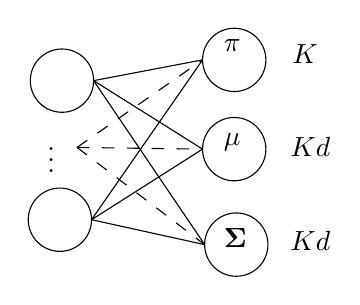
\begin{tikzpicture}[x=0.75pt,y=0.75pt,yscale=-1,xscale=1]
%uncomment if require: \path (0,300); %set diagram left start at 0, and has height of 300

%Shape: Circle [id:dp2684613103597593] 
\draw   (88,112.25) .. controls (88,103.83) and (94.83,97) .. (103.25,97) .. controls (111.67,97) and (118.5,103.83) .. (118.5,112.25) .. controls (118.5,120.67) and (111.67,127.5) .. (103.25,127.5) .. controls (94.83,127.5) and (88,120.67) .. (88,112.25) -- cycle ;
%Shape: Circle [id:dp7515334993320522] 
\draw   (87,179.25) .. controls (87,170.83) and (93.83,164) .. (102.25,164) .. controls (110.67,164) and (117.5,170.83) .. (117.5,179.25) .. controls (117.5,187.67) and (110.67,194.5) .. (102.25,194.5) .. controls (93.83,194.5) and (87,187.67) .. (87,179.25) -- cycle ;
%Shape: Circle [id:dp3956810510931634] 
\draw   (171,102.25) .. controls (171,93.83) and (177.83,87) .. (186.25,87) .. controls (194.67,87) and (201.5,93.83) .. (201.5,102.25) .. controls (201.5,110.67) and (194.67,117.5) .. (186.25,117.5) .. controls (177.83,117.5) and (171,110.67) .. (171,102.25) -- cycle ;
%Shape: Circle [id:dp19016463396194694] 
\draw   (171,145.25) .. controls (171,136.83) and (177.83,130) .. (186.25,130) .. controls (194.67,130) and (201.5,136.83) .. (201.5,145.25) .. controls (201.5,153.67) and (194.67,160.5) .. (186.25,160.5) .. controls (177.83,160.5) and (171,153.67) .. (171,145.25) -- cycle ;
%Shape: Circle [id:dp22276868355052848] 
\draw   (172,191.25) .. controls (172,182.83) and (178.83,176) .. (187.25,176) .. controls (195.67,176) and (202.5,182.83) .. (202.5,191.25) .. controls (202.5,199.67) and (195.67,206.5) .. (187.25,206.5) .. controls (178.83,206.5) and (172,199.67) .. (172,191.25) -- cycle ;
%Straight Lines [id:da20531398432018322] 
\draw    (118.5,112.25) -- (171,102.25) ;
%Straight Lines [id:da5015846339156749] 
\draw    (118.5,112.25) -- (171,145.25) ;
%Straight Lines [id:da38303527040684293] 
\draw    (118.5,112.25) -- (172,191.25) ;
%Straight Lines [id:da4507480129941899] 
\draw    (117.5,179.25) -- (171,102.25) ;
%Straight Lines [id:da05738820526860411] 
\draw    (117.5,179.25) -- (171,145.25) ;
%Straight Lines [id:da686450750606536] 
\draw    (117.5,179.25) -- (172,191.25) ;
%Straight Lines [id:da31471436513544004] 
\draw  [dash pattern={on 4.5pt off 4.5pt}]  (110.5,144.43) -- (171,102.25) ;
%Straight Lines [id:da4379798871611733] 
\draw  [dash pattern={on 4.5pt off 4.5pt}]  (110.5,144.43) -- (171,145.25) ;
%Straight Lines [id:da5452061589510788] 
\draw  [dash pattern={on 4.5pt off 4.5pt}]  (110.5,144.43) -- (172,191.25) ;

% Text Node
\draw (95,135.4) node [anchor=north west][inner sep=0.75pt]    {$\vdots $};
% Text Node
\draw (180,91) node [anchor=north west][inner sep=0.75pt]   [align=left] {$\displaystyle \mathbf{\pi }$};
% Text Node
\draw (180,136.4) node [anchor=north west][inner sep=0.75pt]    {$\mathbf{\mu }$};
% Text Node
\draw (180,182.4) node [anchor=north west][inner sep=0.75pt]    {$\mathbf{\Sigma }$};
% Text Node
\draw (212,138.4) node [anchor=north west][inner sep=0.75pt]    {$Kd$};
% Text Node
\draw (212,183.4) node [anchor=north west][inner sep=0.75pt]    {$Kd$};
% Text Node
\draw (213,93.4) node [anchor=north west][inner sep=0.75pt]    {$K$};


\end{tikzpicture}
\caption{A mixture density output layer. }
\end{figure}

\subsection{MDRNNs and Dreams}

MDRNNs combine both intermediate recurrent layers and an MDN output layer as depicted in Figure \ref{memFig}. 
Their stochastic output makes them great candidates for generative sequence prediction and they have seen a variety of applications, including in systems that complete human sketches \citep{ha2017neural} or compose responses to human generated music \citep{martin2018robojam}.
In standard sequence prediction an RNN reads in a sequence and at each timestep learns to predict what the next element of the sequence will be.
MDRNNs operate on basically the same principle except they generate a probability distribution of the next sequence element and thus allow for stochastic generation of different sequences from the same starting point.

% \begin{figure}[h]
%   \centering
%   \includegraphics[scale=0.2]{catssketch.png}
% \end{figure}

In World Models the MDRNN $M$ engages in a form of sequence prediction.
Given a sequence of latent states $(z_t)$ and actions $(a_t)$, it is trained to predict the distribution $p(z_{t+1} | z_t, a_t, h_t)$.
Once training is complete we follow a simple algorithm in order to generate a dream:
\begin{enumerate}
  \item Choose an initial $z_0$ either randomly or from the start of a real sequence 
  \item Set $h_0 := 0$ and $t:=0$
  \item Repeat for the duration of the dream:
  \begin{enumerate}
    \item Choose an action $a_t$ from a policy or human interaction
    \item Compute $p(z_{t+1} | z_t, a_t, h_t)$ and let $h_{t+1}$ be the output of the LSTM layer
    \item Sample $z_{t+1}$ from $p(z_{t+1} | z_t, a_t, h_t)$
    \item Set $t := t+1$
  \end{enumerate}
\end{enumerate}
Dreams can be rendered in real time by putting each generated latent vector into the $V$'s decoder to make them resemble image observations.
In step 3c a variance controlling term $\tau$ can be used to encourage more chaotic dreams.
David Ha recommends this term be increased for agents trained entirely inside dreams to prevent overfitting from an agent learning to exploit the dream.

In addition to the compressed representation making the sequence dynamics easier to learn the use of the VAE has a second advantage.
Since the encoder learns a probability distribution its encoding are necessarily noisy and so the decoder learns to be robust with respect to its inputs.
Thus mildly unrealistic latent vectors $z_t$ in the dream sequence don't result in complete decoherence as the decoder is still able to make them look somewhat reasonable.
It is this feature that enables the long term stability of World Models dreams.

\section{Controller}
The Controller $C$ is the part of the World Models agent that actually makes decisions.
It takes in the current latent state $z_t$ from $V$ and the current internal state $h_{t-1}$ from $M$ and uses these to decide on an action $a_t$.
In fact the action is chosen using a simple learned linear model
$$a_t = W_C [z_t, h_t] + b_C$$
with an action-space specific activation function.
At first glance it might seem like a linear model is overly simplistic, however the beauty of the World Models' architecture is that it offloads the complexity of the agent into the $V$ and $M$ components.
We can think of these components as unsupervised feature extraction techniques as they effectively learn to output highly relevant predictive features of the environment.
Equipped with these features $C$ is able to harness the information they contain about environment dynamics, rather than learning its own complex relationship between observations, decisions and rewards.

The benefit of using a simpler controller is that it avoids the credit assignment problem mentioned in the introduction.
Less weights to learn means searching the weight space is easier, and by using a single layer we don't have to deal with the vanishing gradient problems which plague deep reinforcement learning models.
In fact the Controller's weight space is small enough that we don't need to employ traditional gradient methods at all.
Instead $C$ is trained using an evolutionary algorithm known as Covariance Matrix Adaptation Evolutionary Strategy (CMA-ES).
In each \textit{generation} of this algorithm a population of agents is sampled from a normal distribution over the weight space of the Controller.
Each member of the population participates in several trial rollouts of the environment.
A certain proportion of the population's best performing or ``fittest'' agents are selected and their weights are used to update the mean and covariance of the normal distribution for the next generation.
CMA-ES is a relatively sophisticated evolutionary algorithm and its advantage over more simplistic methods is that by adjusting its covariance matrix it can explore more widly when the fittest solutions are more far apart and exploit more narrowly if they are closer together.


\begin{figure}[h]
  \centering
  \begin{minipage}{0.4\textwidth}
      \centering
      \includegraphics[width=0.9\textwidth]{cmaes_step1.png} % first figure itself
      \caption{CMA-ES: A narrow population resulting from a smaller covariance matrix (Credit: \cite{ha2017visual}) }
  \end{minipage}\hfill
  \begin{minipage}{0.4\textwidth}
      \centering
      \includegraphics[width=0.9\textwidth]{cmaes_step4.png} % second figure itself
      \caption{CMA-ES: A wider population resulting from a larger covariance matrix (Credit: \cite{ha2017visual})} 
  \end{minipage}
\end{figure}




\section{Implementation}
I wrote a replication of the $V$ and $M$ components of World Models.
I trained and tested these models in the \texttt{CarRacing-v0} environment as well as a \texttt{SimCity-Snes} environment that I built within OpenAI's gym retro system \citep{nichol2018retro}.

\subsection{OpenAI Gym}
OpenAI Gym \citep{gym} is an open source interface for reinforcement learning environments.
It implements an environment class \texttt{Env} which encapsulates the information in an environment such as observations, actions, rewards, etc.
This object-oriented design makes it easy to write code for arbitrary environments as we can reuse common structures like rollout loops.
Environments are simulated frame by frame and the programmer chooses when to advance to the next frame using the \texttt{.step()} method which also returns the next observation and reward as well as other information.
This design means that environments can be run in faster than real time during rollouts or training, but also stepped through slowly for debugging purposes.
All environments include a \texttt{.render()} method which allows us to visualise their state.

\lstset{style=pystyle}
\begin{figure}[h]
\begin{lstlisting}[language=Python]
  import gym
  env = gym.make("CarRacing-v0")
  observation = env.reset()
  for _ in range(1000):
    env.render()
    action = env.action_space.sample() # your agent here (this takes random actions)
    observation, reward, done, info = env.step(action)
  
    if done:
      observation = env.reset()
  env.close()
\end{lstlisting}
\caption{A basic rollout loop for the \texttt{CarRacing-v0} environment}
\end{figure}

Gym is packaged with a number of default environments which can pretty much be used out of the box.
The \texttt{CarRacing-v0} environment is one such environment, coming in the \texttt{Box2D} environment collection, and I used this in my implementation.
A leaderboard of model performance is hosted \href{https://github.com/openai/gym/wiki/Leaderboard}{here} and as of the time of writing David Ha still holds the record in \texttt{CarRacing-v0}.
It is also possible to write custom Gym environments and it has become somewhat of a defacto standard in the reinforcement learning community to implement RL environments this way.
The \texttt{VizDoom: Take Cover} environment used in World Models is also a gym environment.

\subsection{Gym Retro}

Gym Retro \citep{nichol2018retro} is a project which turns old videogames into gym environments.
Retro interfaces with console emulators supporting the \href{https://www.libretro.com/index.php/api/}{Libretro API} to run the games and currently supports a variety of Nintendo, Atari, NEC, and Sega consoles.
Environments within Retro must be partially human created in a process known as integration.
This involves defining a starting state for the environment as well as a reward function and finishing condition.
By default observations are screen images and actions are button presses, however custom choices are possible.
Retro provides a fantastic integration UI which is used to search game memory for variables such as score or lives to base the reward function on.

\begin{figure}[h]
  \centering
  \includegraphics[scale=0.15]{integrationUI.png}
  \caption{SimCity in the Retro integration UI}
\end{figure}

I used the integration UI to make my own integration of the 1991 game SimCity\footnote{Originally I had planned to use the \texttt{gym-city} environment but I found it to be extremely buggy and lacking documentation.} released on the Super Nintendo Entertainment System (SNES).
In SimCity the player is tasked with planning a functioning city on a square grid map.
The player designates zones for residential, commercial, or industrial constructions and lays down infrastructure such as roads, railways, and powerlines.
The city grows acccording to complex cellular-automaton-like rules and the player must add to it and adapt it as issues arise.
In my integration I defined the starting state to be a completely unbuilt city.
I used the default image based observations as well as observations corresponding to the city's population and budget which I used the integration UI to locate in game memory.
One thing to note here is that SimCity actually counts population in multiples of 10 so to find the population I had to search game memory for a value one tenth of the displayed valued.
As a reward function I chose population delta, with the ultimate goal of reaching 10,000 population.

Unfortunately I was unable to get my integration to run as a gym environment due to a \href{https://github.com/openai/retro/issues/115}{bug} which appears to be specific to the SNES emulator used.
Essentially Retro was only able to access game memory inside the integration UI and not inside the gym environment.
This meant that the environment would crash whenever I queried it for memory information.
In addition to making it impossible to define a reward function this meant I was not able to implement custom actions to circumvent the difficulty of learning to navigate the in game UI by button presses.
Ultimately I ended up using a severely reduced environment which started with a preplanned but undeveloped city and simply recorded its growth.



\subsection{The VAE}
\label{VAEsubsec}
%Exact architectures
In the World Models experiments each image observation was a $64\times 64$ image with three colour channels.
The encoder consisted of four RELU convolutional layers connected to a dense output which learned to represent a 32 dimensional Gaussian.
The decoder had a dense layer with 1024 neurons followed by four RELU deconvolutional layers.
I built a VAE in Keras \citep{chollet2015keras} following a very helpful \href{https://tiao.io/post/tutorial-on-variational-autoencoders-with-a-concise-keras-implementation/}{tutorial} and adapting the network architecture to the desired shape.
For the initial experiment with \texttt{CarRacing-v0} I copied the World Models architecture exactly.
In the subsequent experiment with \texttt{SimCity-Snes} I had to adapt the VAE to deal with the larger $160 \times 90$ images.
To do this I used six convolutional and deconvolutional layers instead of four, with rectangular kernels for the deconvolutional layers.
I decided to keep the dimensions of the dense and latent layers the same, to maintain the ease of learning dynamics of the latent variable, however this was something I would have liked to experiment with given more time.

\begin{figure}[h]
  \centering
  \includegraphics[scale=0.4]{vae_arch.png}
  \caption{The original World Models VAE architecture (Credit: \cite{ha2018world})}
  \label{vaeArchFig}
\end{figure}

In World Models David Ha trains the VAE for \texttt{CarRacing-v0} by collecting 10,000 random rollouts of the environment and then learning with gradient descent for only one epoch.
Due to memory constraints I used only 100 random rollouts but trained for 1000 epochs.
In hinsight I should have been more thorough here and used a test set to check for overfitting.
I also used a modified policy to encourage acceleration at the beginning of rollouts to more fully explore the environment.
Since the \texttt{CarRacing-v0} environment actually returns $96 \times 96$ pixel images I used \texttt{tensorflow.Image.resize()} to resize them to $64 \times 64$ pixels.
With \texttt{SimCity-v0} environmental change is much more long term so I recorded one long epsiode (about 5 minute of in game time).
Since the images being learned were more complex I trained for 4000 epochs.

%Training graph

% \begin{figure}[h]
%   \centering
%   \begin{minipage}{0.3\textwidth}
%       \centering
%       \includegraphics[width=0.9\textwidth]{epoch_kl_loss.svg} % first figure itself
%       \caption{Epoch KL loss}
%   \end{minipage}\hfill
%   \begin{minipage}{0.3\textwidth}
%       \centering
%       \includegraphics[width=0.9\textwidth]{epoch_reconstruction_loss.svg} % second figure itself
%       \caption{Epoch reconstruction loss}
%   \end{minipage}
%   \begin{minipage}{0.3\textwidth}
%     \centering
%     \includegraphics[width=0.9\textwidth]{epoch_loss.svg} % second figure itself
%     \caption{Epoch combined loss}
% \end{minipage}
% \end{figure}

In the \texttt{CarRacing-v0} environment the reconstructed images from my VAE were visually indistinguishable from the originals.
By contrast the images from \texttt{SimCity-Snes} were visually similar to the originals but had noticeably imperfections.
I attribute this difference to the fact that the \texttt{SimCity-Snes} observations were both higher dimensional and more visually complex and suspect that it could have been adressed by increasing the dimension of the latent variable and hidden dense layers.
For both experiments I tried generating new images by sampling from a zero mean unit variance Gaussian and feeding it to the trained decoder.
The images generated for \texttt{CarRacing-v0} visually somewhat visually resembled the environment but contained glitches such as disconnected tracks or even patches of black learned from the game's initial black border.
The images generated for \texttt{SimCity-Snes} also resembled the game, with the most obvious visual glitch being incorrect colours palettes, which presumably arise as a form of confusion between the game's different seasonal colour palettes.

%reconstruction pictures
\begin{figure}
  \centering
  \begin{minipage}{0.45\textwidth}
      \centering
      \includegraphics[width=0.9\textwidth]{287_before.png} % first figure itself
  \end{minipage}\hfill
  \begin{minipage}{0.45\textwidth}
      \centering
      \includegraphics[width=0.9\textwidth]{287_after.png} % second figure itself
  \end{minipage}
  \caption{Observation and VAE reconstructed image for \texttt{CarRacing-v0}}
\end{figure}

% VAE generative pictures
\begin{figure}
  \centering
  \begin{minipage}{0.3\textwidth}
      \centering
      \includegraphics[width=0.9\textwidth]{gen_im3.png} % first figure itself
  \end{minipage}\hfill
  \begin{minipage}{0.3\textwidth}
      \centering
      \includegraphics[width=0.9\textwidth]{gen_im1.png} % second figure itself
  \end{minipage}\hfill
  \begin{minipage}{0.3\textwidth}
    \centering
    \includegraphics[width=0.9\textwidth]{gen_im2.png} % second figure itself
\end{minipage}
\caption{Randomly generated images for \texttt{CarRacing-v0}}
\end{figure}

\begin{figure}
  \centering
  \begin{minipage}{0.45\textwidth}
      \centering
      \includegraphics[width=\textwidth]{obs_24.png} % first figure itself
  \end{minipage}\hfill
  \begin{minipage}{0.45\textwidth}
      \centering
      \includegraphics[width=\textwidth]{recon_24.png} % second figure itself
  \end{minipage}
  \caption{Observation and VAE reconstructed image for \texttt{SimCity-Snes}}
\end{figure}

\begin{figure}
  \centering
  \begin{minipage}{0.45\textwidth}
      \centering
      \includegraphics[width=\textwidth]{gen_im5.png} % first figure itself
  \end{minipage}\hfill
  \begin{minipage}{0.45\textwidth}
      \centering
      \includegraphics[width=\textwidth]{gen_im4.png} % second figure itself
  \end{minipage}
  \caption{Randomly generated images for \texttt{SimCity-Snes}}
\end{figure}

\subsection{The MDRNN}
\label{MDRNNsubsec}
As mentioned earlier the MDRNNs in World Models consisted of an LSTM input layer and MDN output.
For \texttt{CarRacing-v0} they used 256 hidden memory cells and for \texttt{VizDoom: Take Cover} they used 512.
In both experiments they used five mixture components for the MDN output.
I implemented the MDRNN using Keras' built in LSTM layer and a \href{https://github.com/cpmpercussion/keras-mdn-layer}{Keras MDN layer} written by my supervisor.
For both of my experiments I used 256 memory cells and 5 mixture components.
The use of more mixture components and memory cells to capture more complex dynamics was something I would have liked to experiment more with given time.

To train the MDRNN the already trained $V$ component is used to preprocess the existing rollouts into latent representations.
Rather than storing a single latent vector $z$ for each original observation we store $\mu$ and $\sigma$.
In training we take a batch of multiple episodes, and unroll the network over each episode.
In each training batch we sample latent variables using the stored $\mu$ and $\sigma$ and task the MDRNN with learning to predict these sequences.
By sampling each time we see an episode we avoid overfitting to a single arbitray sampled value.

I did not implement real time interactive dreams but I was able to record footage of dreams under agent policies.
For \texttt{CarRacing-v0} I found the dream comparable in quality to the interactive dream released with World Models.
The model was able to correctly simulate dynamics of the world, including acceleration, turning, and the initial camera zoom.
It did encounter similar decoherence issues where the track would behave unpredictably and once lost would not reappear.
For \texttt{SimCity-v0} the dreams were able to remain relatively coherent but did not learn long term dynamics of the world or such as seasonal change.
I would have liked to experiment with this more by using more powerful hardware to facilitate training on long sequences and more data.


\section{Conclusion and Further Work}
%blah blah I learned a lot
%More things I would have liked to do
%response papers (charles')



\clearpage
\bibliography{ref} 
\end{document}
